\documentclass[10pt,A4,]{article}
% \RequirePackage[l2tabu, orthodox]{nag}
\usepackage[a4paper,text={16.5cm,25.2cm},centering,margin=2.6cm]{geometry}
% \usepackage[left=1.0in,top=1.0in,right=1.0in,bottom=1.0in]{geometry}
\newcommand*{\authorfont}{\fontfamily{phv}\selectfont}
\usepackage{hyperref,amsmath,amssymb,bm,url,enumitem,dcolumn,upquote,framed,alltt,textgreek,xfrac,fixltx2e}
\usepackage[australian]{babel}
\usepackage[compact,small]{titlesec}
\setlength{\parskip}{1.2ex}
\setlength{\parindent}{0em}

\def\tightlist{}

\usepackage{ifxetex}
\ifxetex
  \usepackage{fontspec}
  \defaultfontfeatures{Ligatures=TeX} % To support LaTeX quoting style
 \defaultfontfeatures{Ligatures=TeX}
 \setmainfont{Minion Pro}
 \setsansfont[Scale=MatchLowercase]{Myriad Pro}
 \setmonofont[Scale=MatchLowercase]{Ubuntu Mono}
\else
  \usepackage[T1]{fontenc}
  \usepackage[utf8]{inputenc}
  \usepackage{lmodern}
  % \usepackage[full]{textcomp} % directly use the degree (and some other) symbol
\fi

% place after fonts; even better typesetting for improved readability:
% \graphicspath{ {figure/} }
\usepackage{tabularx} % for 'tabularx' environment and 'X' column type
\usepackage{ragged2e}  % for '\RaggedRight' macro (allows hyphenation)
\usepackage{siunitx}
    \sisetup{%
        detect-mode,
        group-digits            = false,
        input-symbols           = ( ) [ ] - + < > *,
        table-align-text-post   = false,
        round-mode              = places,
        round-precision         = 3
        }
% \usepackage[font={small, sf}, labelfont=bf]{caption} % tweaking the captions
\usepackage[font={small}, labelfont=bf]{caption} % tweaking the captions
\usepackage[color=yellow, textsize=tiny]{todonotes}
\frenchspacing%
% \usepackage[kerning=false,protrusion=true,expansion=true]{microtype}

\usepackage{abstract}
\renewcommand{\abstractname}{} % clear the title
\renewcommand{\absnamepos}{empty} % originally center

\renewenvironment{abstract}
{{%
\setlength{\leftmargin}{0mm}
\setlength{\rightmargin}{\leftmargin}%
}%
\relax}
{\endlist}

\makeatletter
\def\@maketitle{%
\newpage
%  \null
%  \vskip 2em%
%  \begin{center}%
\let \footnote \thanks
 {\fontsize{18}{20}\selectfont\raggedright  \setlength{\parindent}{0pt} \@title \par}%
}
%\fi
\makeatother


\setcounter{secnumdepth}{0}



\usepackage{color}
\usepackage{fancyvrb}
\newcommand{\VerbBar}{|}
\newcommand{\VERB}{\Verb[commandchars=\\\{\}]}
\DefineVerbatimEnvironment{Highlighting}{Verbatim}{commandchars=\\\{\}}
% Add ',fontsize=\small' for more characters per line
\usepackage{framed}
\definecolor{shadecolor}{RGB}{248,248,248}
\newenvironment{Shaded}{\begin{snugshade}}{\end{snugshade}}
\newcommand{\KeywordTok}[1]{\textcolor[rgb]{0.13,0.29,0.53}{\textbf{#1}}}
\newcommand{\DataTypeTok}[1]{\textcolor[rgb]{0.13,0.29,0.53}{#1}}
\newcommand{\DecValTok}[1]{\textcolor[rgb]{0.00,0.00,0.81}{#1}}
\newcommand{\BaseNTok}[1]{\textcolor[rgb]{0.00,0.00,0.81}{#1}}
\newcommand{\FloatTok}[1]{\textcolor[rgb]{0.00,0.00,0.81}{#1}}
\newcommand{\ConstantTok}[1]{\textcolor[rgb]{0.00,0.00,0.00}{#1}}
\newcommand{\CharTok}[1]{\textcolor[rgb]{0.31,0.60,0.02}{#1}}
\newcommand{\SpecialCharTok}[1]{\textcolor[rgb]{0.00,0.00,0.00}{#1}}
\newcommand{\StringTok}[1]{\textcolor[rgb]{0.31,0.60,0.02}{#1}}
\newcommand{\VerbatimStringTok}[1]{\textcolor[rgb]{0.31,0.60,0.02}{#1}}
\newcommand{\SpecialStringTok}[1]{\textcolor[rgb]{0.31,0.60,0.02}{#1}}
\newcommand{\ImportTok}[1]{#1}
\newcommand{\CommentTok}[1]{\textcolor[rgb]{0.56,0.35,0.01}{\textit{#1}}}
\newcommand{\DocumentationTok}[1]{\textcolor[rgb]{0.56,0.35,0.01}{\textbf{\textit{#1}}}}
\newcommand{\AnnotationTok}[1]{\textcolor[rgb]{0.56,0.35,0.01}{\textbf{\textit{#1}}}}
\newcommand{\CommentVarTok}[1]{\textcolor[rgb]{0.56,0.35,0.01}{\textbf{\textit{#1}}}}
\newcommand{\OtherTok}[1]{\textcolor[rgb]{0.56,0.35,0.01}{#1}}
\newcommand{\FunctionTok}[1]{\textcolor[rgb]{0.00,0.00,0.00}{#1}}
\newcommand{\VariableTok}[1]{\textcolor[rgb]{0.00,0.00,0.00}{#1}}
\newcommand{\ControlFlowTok}[1]{\textcolor[rgb]{0.13,0.29,0.53}{\textbf{#1}}}
\newcommand{\OperatorTok}[1]{\textcolor[rgb]{0.81,0.36,0.00}{\textbf{#1}}}
\newcommand{\BuiltInTok}[1]{#1}
\newcommand{\ExtensionTok}[1]{#1}
\newcommand{\PreprocessorTok}[1]{\textcolor[rgb]{0.56,0.35,0.01}{\textit{#1}}}
\newcommand{\AttributeTok}[1]{\textcolor[rgb]{0.77,0.63,0.00}{#1}}
\newcommand{\RegionMarkerTok}[1]{#1}
\newcommand{\InformationTok}[1]{\textcolor[rgb]{0.56,0.35,0.01}{\textbf{\textit{#1}}}}
\newcommand{\WarningTok}[1]{\textcolor[rgb]{0.56,0.35,0.01}{\textbf{\textit{#1}}}}
\newcommand{\AlertTok}[1]{\textcolor[rgb]{0.94,0.16,0.16}{#1}}
\newcommand{\ErrorTok}[1]{\textcolor[rgb]{0.64,0.00,0.00}{\textbf{#1}}}
\newcommand{\NormalTok}[1]{#1}


\usepackage{longtable,booktabs}
\setlength\heavyrulewidth{0.1em}
\setlength\lightrulewidth{0.0625em}

\usepackage{graphicx}
% We will generate all images so they have a width \maxwidth. This means
% that they will get their normal width if they fit onto the page, but
% are scaled down if they would overflow the margins.
\makeatletter
\def\maxwidth{\ifdim\Gin@nat@width>\linewidth\linewidth
\else\Gin@nat@width\fi}
\makeatother
\let\Oldincludegraphics\includegraphics
\renewcommand{\includegraphics}[1]{\Oldincludegraphics[width=\maxwidth]{#1}}

\title{Quantifying the impact of wind and wave action on seawater temperature
along the South African coastline (Appendices)  }

\author{\Large Amieroh Abrahams\vspace{0.05in} \newline\normalsize\emph{University of the Western Cape}  }

\date{}

% PENALTIES
\widowpenalty=1000
\clubpenalty=1000
\doublehyphendemerits=9999 % Almost no consecutive line hyphens
\brokenpenalty=10000 % No broken words across columns/pages
\interfootnotelinepenalty=9999 % Almost never break footnotes

% SECTION, SUBSECETC.TITLES
\usepackage[compact]{titlesec}
\titleformat{\chapter}
  {\normalfont\LARGE\sffamily\bfseries}
  {\thechapter}
  {1em}
  {}
\titleformat{\section}
  {\normalfont\LARGE\sffamily\bfseries}
  {\thesection}
  {1em}
  {}
\titleformat{\subsection}
  {\normalfont\Large\sffamily\bfseries}
  {\thesubsection}
  {1em}
  {}
\titleformat{\subsubsection}
  {\normalfont\large\sffamily\bfseries\slshape}
  {\thesubsubsection}
  {1em}
  {}
% \titlespacing*{<command>}{<left>}{<before-sep>}{<after-sep>}
\titlespacing*{\chapter}
  {0pt}
  {1.2ex plus 1ex minus .2ex}
  {0.5ex plus .1ex minus .1ex}
\titlespacing*{\section}
  {0pt}
  {1.2ex plus 1ex minus .2ex}
  {0.5ex plus .1ex minus .1ex}
\titlespacing*{\subsection}
  {0pt}
  {1.2ex plus 1ex minus .2ex}
  {0.5ex plus .1ex minus .1ex}
\titlespacing*{\subsubsection}
  {0pt}
  {1.2ex plus 1ex minus .2ex}
  {0.5ex plus .1ex minus .1ex}



\newtheorem{hypothesis}{Hypothesis}
\usepackage{setspace}

\makeatletter

\@ifpackageloaded{hyperref}{}{%
\ifxetex
  \usepackage[setpagesize=false, % page size defined by xetex
              unicode=false, % unicode breaks when used with xetex
              xetex]{hyperref}
\else
  \usepackage[colorlinks=true, citecolor=blue, linkcolor=cyan, pdfborder={0 0 0 }, unicode=true]{hyperref} % place after other packages, but before cleveref
\fi
}

\@ifpackageloaded{color}{
    \PassOptionsToPackage{usenames,dvipsnames}{color}
}{%
    \usepackage[usenames,dvipsnames]{color}
}

\usepackage{cleveref} % cleverly cross referencing figures and tables; last package to include
\setcounter{secnumdepth}{2}
\setcounter{tocdepth}{2}

% To use for resetting the numbering of Appendix Tables and Figures:
%\setcounter{table}{0}
%\renewcommand{\thetable}{A\arabic{table}}
%\setcounter{figure}{0}
%\renewcommand{\thefigure}{A\arabic{figure}}

\makeatother
\hypersetup{breaklinks=true,
            bookmarks=true,
            pdfauthor={Amieroh Abrahams (University of the Western Cape)},
             pdfkeywords = {},
            pdftitle={Quantifying the impact of wind and wave action on seawater temperature
along the South African coastline (Appendices)},
            colorlinks=true,
            citecolor=blue,
            urlcolor=blue,
            linkcolor=magenta,
            pdfborder={0 0 0}}
\urlstyle{same}  % don't use monospace font for urls


\begin{document}

% \maketitle

{% \usefont{T1}{pnc}{m}{n}
\setlength{\parindent}{0pt}
\thispagestyle{plain}
{\fontsize{18}{20}\selectfont\raggedright
\maketitle  % title \par
}
{
   \vskip 13.5pt\relax \normalsize\fontsize{11}{12}
\textbf{\authorfont Amieroh Abrahams} \hskip 15pt \emph{\small University of the Western Cape}   
}
}



\vskip 6.5pt

\noindent 

This file was generated in R using Rmarkdown, with a bit of
\LaTeX~thrown in:

\begin{Shaded}
\begin{Highlighting}[]
\KeywordTok{sessionInfo}\NormalTok{()}
\end{Highlighting}
\end{Shaded}

\begin{verbatim}
## R version 3.5.0 (2018-04-23)
## Platform: x86_64-apple-darwin15.6.0 (64-bit)
## Running under: macOS  10.14.1
## 
## Matrix products: default
## BLAS: /Library/Frameworks/R.framework/Versions/3.5/Resources/lib/libRblas.0.dylib
## LAPACK: /Library/Frameworks/R.framework/Versions/3.5/Resources/lib/libRlapack.dylib
## 
## locale:
## [1] en_US.UTF-8/en_US.UTF-8/en_US.UTF-8/C/en_US.UTF-8/en_US.UTF-8
## 
## attached base packages:
## [1] stats     grDevices utils     datasets  graphics  methods   base     
## 
## loaded via a namespace (and not attached):
##  [1] compiler_3.5.0  backports_1.1.2 magrittr_1.5    rprojroot_1.3-2
##  [5] tools_3.5.0     htmltools_0.3.6 yaml_2.2.0      Rcpp_1.0.0     
##  [9] stringi_1.2.4   rmarkdown_1.10  knitr_1.20      stringr_1.3.1  
## [13] digest_0.6.18   evaluate_0.12
\end{verbatim}

\newpage

\section*{\large{Appendix A}}

\subsection*{Background and code}

The intention of this section is to show the approach and \textbf{R}
scripts used to analyse the possible reasons for temperature variation
between sites within the same cluster along the coast of South Africa.
Specifically, I wish to determine if wave and wind action are the
possible reasons for this variation.

\subsubsection*{The data}

The SACTN dataset is the primary source of temperature data used in this
study. This dataset consisted of \emph{in situ} collected coastal
seawater temperatures for 129 sites along the coast of South Africa,
measured daily from 1972 until 2017. This study also make use of AVHRR,
MUR, CMC and K10 satellite-derived SST datasets as well as wind and wave
action data that were obtained from the South African Weather Service
(SAWS), and were provided at three hour resolutions. This data was then
used to model short--crested waves, generated by the wind into the
coastal environment, using the wave model Simulating Waves in the
Nearshore (SWAN).

\subsubsection*{Setting up the analysis}

This is \textbf{R}, so first I need to find, install and load various
packages. Some of the packages will be available on CRAN and can be
accessed and installed in the usual way.

\begin{Shaded}
\begin{Highlighting}[]
\KeywordTok{library}\NormalTok{(tidyverse)}
\end{Highlighting}
\end{Shaded}

\begin{verbatim}
## -- Attaching packages ---------------------------------------------------------------------------------------------- tidyverse 1.2.1 --
\end{verbatim}

\begin{verbatim}
## v ggplot2 3.1.0     v purrr   0.2.5
## v tibble  1.4.2     v dplyr   0.7.8
## v tidyr   0.8.2     v stringr 1.3.1
## v readr   1.1.1     v forcats 0.3.0
\end{verbatim}

\begin{verbatim}
## -- Conflicts ------------------------------------------------------------------------------------------------- tidyverse_conflicts() --
## x dplyr::filter() masks stats::filter()
## x dplyr::lag()    masks stats::lag()
## x dplyr::n()      masks .env::n()
\end{verbatim}

\begin{Shaded}
\begin{Highlighting}[]
\KeywordTok{library}\NormalTok{(ggpubr)}
\end{Highlighting}
\end{Shaded}

\begin{verbatim}
## Loading required package: magrittr
\end{verbatim}

\begin{verbatim}
## 
## Attaching package: 'magrittr'
\end{verbatim}

\begin{verbatim}
## The following object is masked from 'package:purrr':
## 
##     set_names
\end{verbatim}

\begin{verbatim}
## The following object is masked from 'package:tidyr':
## 
##     extract
\end{verbatim}

\begin{Shaded}
\begin{Highlighting}[]
\KeywordTok{library}\NormalTok{(zoo)}
\end{Highlighting}
\end{Shaded}

\begin{verbatim}
## 
## Attaching package: 'zoo'
\end{verbatim}

\begin{verbatim}
## The following objects are masked from 'package:base':
## 
##     as.Date, as.Date.numeric
\end{verbatim}

\begin{Shaded}
\begin{Highlighting}[]
\KeywordTok{library}\NormalTok{(lubridate)}
\end{Highlighting}
\end{Shaded}

\begin{verbatim}
## 
## Attaching package: 'lubridate'
\end{verbatim}

\begin{verbatim}
## The following object is masked from 'package:base':
## 
##     date
\end{verbatim}

\begin{Shaded}
\begin{Highlighting}[]
\KeywordTok{library}\NormalTok{(ggrepel)}
\KeywordTok{library}\NormalTok{(FNN)}
\KeywordTok{library}\NormalTok{(stringr)}
\KeywordTok{library}\NormalTok{(circular)}
\end{Highlighting}
\end{Shaded}

\begin{verbatim}
## 
## Attaching package: 'circular'
\end{verbatim}

\begin{verbatim}
## The following objects are masked from 'package:stats':
## 
##     sd, var
\end{verbatim}

\begin{Shaded}
\begin{Highlighting}[]
\KeywordTok{library}\NormalTok{(broom)}
\KeywordTok{library}\NormalTok{(ggrepel)}
\KeywordTok{library}\NormalTok{(purrr)}
\KeywordTok{library}\NormalTok{(stlplus)}
\KeywordTok{source}\NormalTok{(}\StringTok{"../functions/earthdist.R"}\NormalTok{)}
\KeywordTok{source}\NormalTok{(}\StringTok{"../functions/scale.bar.func.R"}\NormalTok{)}
\end{Highlighting}
\end{Shaded}

\begin{verbatim}
## 
## Attaching package: 'maps'
\end{verbatim}

\begin{verbatim}
## The following object is masked from 'package:purrr':
## 
##     map
\end{verbatim}

\begin{verbatim}
## Loading required package: sp
\end{verbatim}

\begin{verbatim}
## Checking rgeos availability: TRUE
\end{verbatim}

\begin{Shaded}
\begin{Highlighting}[]
\KeywordTok{source}\NormalTok{(}\StringTok{"../functions/wind.rose.R"}\NormalTok{)}
\end{Highlighting}
\end{Shaded}

\begin{verbatim}
## Loading required package: RColorBrewer
\end{verbatim}

\begin{Shaded}
\begin{Highlighting}[]
\KeywordTok{source}\NormalTok{(}\StringTok{"../functions/waverose.diagram.R"}\NormalTok{)}
\KeywordTok{source}\NormalTok{(}\StringTok{"../functions/match_func.R"}\NormalTok{)}
\KeywordTok{source}\NormalTok{(}\StringTok{"../functions/seasonal_match.R"}\NormalTok{)}
\KeywordTok{source}\NormalTok{(}\StringTok{"../functions/anova_func.R"}\NormalTok{)}
\KeywordTok{source}\NormalTok{(}\StringTok{"../functions/Load_wave_function.R"}\NormalTok{)}
\end{Highlighting}
\end{Shaded}

\begin{verbatim}
## Parsed with column specification:
## cols(
##   site = col_character(),
##   lon = col_double(),
##   lat = col_double(),
##   site_list = col_character(),
##   wave_7 = col_character(),
##   wave_15 = col_character()
## )
\end{verbatim}

\begin{verbatim}
## 
  |                                                                       
  |                                                                 |   0%
  |                                                                       
  |===                                                              |   5%
  |                                                                       
  |======                                                           |  10%
  |                                                                       
  |=========                                                        |  14%
  |                                                                       
  |============                                                     |  19%
  |                                                                       
  |===============                                                  |  24%
  |                                                                       
  |===================                                              |  29%
  |                                                                       
  |======================                                           |  33%
  |                                                                       
  |=========================                                        |  38%
  |                                                                       
  |============================                                     |  43%
  |                                                                       
  |===============================                                  |  48%
  |                                                                       
  |==================================                               |  52%
  |                                                                       
  |=====================================                            |  57%
  |                                                                       
  |========================================                         |  62%
  |                                                                       
  |===========================================                      |  67%
  |                                                                       
  |==============================================                   |  71%
  |                                                                       
  |==================================================               |  76%
  |                                                                       
  |=====================================================            |  81%
  |                                                                       
  |========================================================         |  86%
  |                                                                       
  |===========================================================      |  90%
  |                                                                       
  |==============================================================   |  95%
  |                                                                       
  |=================================================================| 100%
## 
  |                                                                       
  |                                                                 |   0%
  |                                                                       
  |====                                                             |   6%
  |                                                                       
  |========                                                         |  12%
  |                                                                       
  |===========                                                      |  18%
  |                                                                       
  |===============                                                  |  24%
  |                                                                       
  |===================                                              |  29%
  |                                                                       
  |=======================                                          |  35%
  |                                                                       
  |===========================                                      |  41%
  |                                                                       
  |===============================                                  |  47%
  |                                                                       
  |==================================                               |  53%
  |                                                                       
  |======================================                           |  59%
  |                                                                       
  |==========================================                       |  65%
  |                                                                       
  |==============================================                   |  71%
  |                                                                       
  |==================================================               |  76%
  |                                                                       
  |======================================================           |  82%
  |                                                                       
  |=========================================================        |  88%
  |                                                                       
  |=============================================================    |  94%
  |                                                                       
  |=================================================================| 100%
## 
  |                                                                       
  |                                                                 |   0%
  |                                                                       
  |================================                                 |  50%
  |                                                                       
  |=================================================================| 100%
## 
  |                                                                       
  |                                                                 |   0%
  |                                                                       
  |================================                                 |  50%
  |                                                                       
  |=================================================================| 100%
\end{verbatim}

\begin{verbatim}
## Joining, by = "site"
\end{verbatim}

\begin{Shaded}
\begin{Highlighting}[]
\KeywordTok{source}\NormalTok{(}\StringTok{"../functions/R_func.R"}\NormalTok{)}
\KeywordTok{source}\NormalTok{(}\StringTok{"../functions/temp_r2.R"}\NormalTok{)}
\KeywordTok{source}\NormalTok{(}\StringTok{"../functions/temp_wave_r2.R"}\NormalTok{)}
\end{Highlighting}
\end{Shaded}

\newpage

\section*{\large{Appendix B}}

Now to get to the data. Here I load the site list dataset. This dataset
comprise of the statistical properties of the seawater temperature
representing the South African coastline, such as the mean, minimum and
maximum temperatures. These values vary among coastal sections due to
the influence of the cold Benguala and warm Agulhas currents. At the
broad scale, this region exhibits a large variation in seawater
temperatures along its coastline (Mead et al. 2013; Smit et al. 2013)
and is divided into four bioregions, each with contrasting temperatures.
These bioregions are the Benguela Marrine Province (BMP),
Benguela-Agulhas Transition Zone (B-ATZ), the Agulhas Marine Province
(AMP) and the East Coast Transition Zone (ECTZ) (Smit, Bolton, and
Anderson 2017). The Benguela Marine Province (BMP) is located to the
west of Cape Point and is characterized by the movement of cold water
from the Southern Ocean moving north. The cold temperate west coast
mentioned above is greatly affected by the upwelling caused by offshore
winds, generated by the cold Benguela current. Thus the seawater
temperatures found around South Africa's coastline exhibits a large
variational range. My plotting functions partition the data into the
clusters and colour code each point accordingly so that I am able to see
patterns that exist and distictly group the different sites with similar
temperatures along the three distinct coasts.

\begin{Shaded}
\begin{Highlighting}[]
\KeywordTok{load}\NormalTok{(}\StringTok{"../data/site_list_v4.2.RData"}\NormalTok{)}
\end{Highlighting}
\end{Shaded}

\newpage

The next step involves SACTN temperature dataset. First I compute a
k-means clustering on a data matrix using the \texttt{kmeans()}
function, which uses multiple random seeds to find a number of clusting
solutions. This groups sites based on minimum, maximum and mean
temperatures. Thereafter I select all the sites with a overlapping time
series of at least 10 years of data and excluding temperatures collected
deeper than 5m.

\begin{Shaded}
\begin{Highlighting}[]
\KeywordTok{load}\NormalTok{(}\StringTok{"../SACTN_data/SACTN_daily_v4.2.RData"}\NormalTok{)}

\KeywordTok{set.seed}\NormalTok{(}\DecValTok{10}\NormalTok{)}
\NormalTok{site_list}\OperatorTok{$}\NormalTok{cluster <-}\StringTok{ }\KeywordTok{as.factor}\NormalTok{(}\KeywordTok{kmeans}\NormalTok{(site_list[,}\KeywordTok{c}\NormalTok{(}\DecValTok{15}\NormalTok{, }\DecValTok{18}\OperatorTok{:}\DecValTok{19}\NormalTok{)], }\DecValTok{6}\NormalTok{)}\OperatorTok{$}\NormalTok{cluster)}

\NormalTok{site_list_clusters <-}\StringTok{ }\NormalTok{site_list }\OperatorTok\StringTok{ }
\StringTok{  }\KeywordTok{filter}\NormalTok{(length }\OperatorTok{>=}\StringTok{ }\DecValTok{3650}\NormalTok{, depth }\OperatorTok{<=}\StringTok{ }\DecValTok{5}\NormalTok{)}

\NormalTok{SACTN_daily_clusters <-}\StringTok{ }\NormalTok{SACTN_daily_v4.}\DecValTok{2} \OperatorTok\StringTok{ }
\StringTok{  }\KeywordTok{left_join}\NormalTok{(site_list[,}\KeywordTok{c}\NormalTok{(}\DecValTok{4}\NormalTok{, }\DecValTok{13}\NormalTok{, }\DecValTok{21}\NormalTok{)], }\DataTypeTok{by =} \StringTok{"index"}\NormalTok{) }\OperatorTok\StringTok{ }
\StringTok{  }\KeywordTok{filter}\NormalTok{(index }\OperatorTok\StringTok{ }\NormalTok{site_list_clusters}\OperatorTok{$}\NormalTok{index)}
\end{Highlighting}
\end{Shaded}

With the sites now split into eight clusters, the next step is to reduce
the number of sites per cluster down to a manageable, but still
representative, sub-sample of the whole. This is done primarily for two
reasons. The first, simply, is to allow for the comparisons to be more
readily interpretable by humans. The second more objective reason is to
allow for an equal amount of sampling per cluster. The East coast is
much more heavily sampled than the rest and so this imbalance must be
addressed. The criteria that must be considered for the sub-samples are
that both instrument types (UTR and thermometer) are present, and as
many sources are included as are possible. This thermal data contain
various variables, in this study I only make use of some of them. This
resulted in 18 sites, three per cluster. My plotting functions partition
the data into its respective groups and colour code the figures
accordingly.

\begin{Shaded}
\begin{Highlighting}[]
\CommentTok{# Read in the species data}
\CommentTok{# Will be provided -- in the data folder as "site_list_sub.RData"}

\CommentTok{# save(site_list_sub, file = "data/site_list_sub.RData")}
\KeywordTok{load}\NormalTok{(}\StringTok{"../data/site_list_sub.RData"}\NormalTok{)}
\NormalTok{SACTN_daily_clusters_sub <-}\StringTok{ }\NormalTok{SACTN_daily_clusters }\OperatorTok\StringTok{   }\CommentTok{#Subsetting the data}
\StringTok{  }\KeywordTok{filter}\NormalTok{(index }\OperatorTok\StringTok{ }\NormalTok{site_list_sub}\OperatorTok{$}\NormalTok{index)}
\CommentTok{# save(SACTN_daily_clusters_sub, file = "data/SACTN_daily_clusters_sub.RData") #Saving the data for later use}
\end{Highlighting}
\end{Shaded}

\begin{tiny}
\begin{center}
\setlength\tabcolsep{4pt}
\begin{longtable}{|r|r|r|l|p{6cm}|}
\caption{The 18 sites along the South African coastline, with approximate GPS coordinates, source and the cluster of which each site belong to based on maximum, minimum and mean temperature} \\

% This is the header for the first page of the table...
\toprule
Cluster & Site & SRC & Lon & Lat  \\
\midrule
\endfirsthead

% This is the header for the second page of the table...
\toprule
Cluster & Site & SRC & Lon & Lat  \\
\midrule
\endhead

% This is the footer for all pages except the last page of the table...
\midrule
\multicolumn{5}{l}{{Continued on Next Page\ldots}} \\
\endfoot

% This is the footer for the last page of the table...
\bottomrule
\endlastfoot

% Now the data...

1 & Hamburg & DEA & 27.49 & -33.29 \\
1 & Eastern Beach & SAWS & 27.92 & -33.02 \\
1 & Orient Beach & SAWS & 27.92 & -33.02 \\
2 & Stilbaai & SAWS & 21.44 & -34.37 \\
2 & Mossel Bay & SAWS & 22.13 & -34.17 \\
2 & Knysna & SAWS & 23.05 & -34.09 \\
3 & Saldanha Bay & SAWS & 17.95 & -33.01 \\
3 & Bordjies & DAFF & 18.46 & -34.32 \\
3 & Gansbaai & SAWS & 19.34 & -34.59 \\
4 & Port Edward & KZNSB & 30.23 & -31.04 \\
4 & T.O. Strand & KZNSB & 30.23 & -31.03 \\
4 & Leisure Bay & KZNSB & 30.25 & -31.02 \\
5 & Port Nolloth & SAWS & 16.87 & -29.25 \\
5 & Lamberts Bay & SAWS & 18.30 & -32.09 \\
5 & Sea Point & SAWS & 18.38 & -33.92 \\
6 & Kalk Bay & SAWS & 18.45 & -34.13 \\
6 & Muizenberg & SAWS & 18.48 & -34.10 \\
6 & Gordons Bay & SAWS & 18.86 & -34.16 \\

\end{longtable}
\end{center}
\end{tiny}

With the temperature data now loaded in, I am now able to calculate the
distance between each of the sites. Here I set up a geographic or
Euclidian distance matrix representing the pairwise distances between
the \(n\) sites (\(D=[d_{ij}]\)). I already have a function for this and
can be found in the folder titled functions.

\begin{Shaded}
\begin{Highlighting}[]
\KeywordTok{load}\NormalTok{(}\StringTok{"../data/sa_coast.Rdata"}\NormalTok{) }\CommentTok{# Coastal data}
\KeywordTok{options}\NormalTok{(}\DataTypeTok{scipen=}\DecValTok{999}\NormalTok{) }\CommentTok{# Forces R to not use exponential notation}
\NormalTok{sa_coast_prep <-}\StringTok{ }\NormalTok{sa_coast }\OperatorTok\StringTok{ }
\StringTok{  }\KeywordTok{mutate}\NormalTok{(}\DataTypeTok{site =} \DecValTok{1}\OperatorTok{:}\KeywordTok{nrow}\NormalTok{(.),}
         \DataTypeTok{X =} \KeywordTok{deg2rad}\NormalTok{(X),}
         \DataTypeTok{Y =} \KeywordTok{deg2rad}\NormalTok{(Y)) }\OperatorTok\StringTok{ }
\StringTok{  }\KeywordTok{select}\NormalTok{(site, X, Y)}

\NormalTok{sa_coast_dist <-}\StringTok{ }\KeywordTok{as.data.frame}\NormalTok{(}\KeywordTok{round}\NormalTok{(}\KeywordTok{PairsDists}\NormalTok{(sa_coast_prep), }\DecValTok{2}\NormalTok{)) }\OperatorTok\StringTok{ }
\StringTok{  }\KeywordTok{mutate}\NormalTok{(}\DataTypeTok{lon =}\NormalTok{ sa_coast}\OperatorTok{$}\NormalTok{X,}
         \DataTypeTok{lat =}\NormalTok{ sa_coast}\OperatorTok{$}\NormalTok{Y) }\OperatorTok\StringTok{ }
\StringTok{  }\NormalTok{dplyr}\OperatorTok{::}\KeywordTok{rename}\NormalTok{(}\DataTypeTok{dist =}\NormalTok{ V1) }\OperatorTok
\StringTok{  }\KeywordTok{select}\NormalTok{(lon, lat, dist) }\OperatorTok\StringTok{ }
\StringTok{  }\KeywordTok{mutate}\NormalTok{(}\DataTypeTok{cum_dist =} \KeywordTok{cumsum}\NormalTok{(dist)) }\OperatorTok\StringTok{ }
\StringTok{  }\KeywordTok{mutate}\NormalTok{(}\DataTypeTok{dist =} \KeywordTok{lag}\NormalTok{(dist),}
         \DataTypeTok{cum_dist =} \KeywordTok{lag}\NormalTok{(cum_dist))}
\end{Highlighting}
\end{Shaded}

\subsubsection*{Matching sites based on overlapping time series}

Next I create a function to match the sites with each of the clusters.
This allows me to compare whether or not a temperature variation exist
between sites within the same cluster and to examine reasons for this
variation. Here I also consider distance between sites.

\begin{Shaded}
\begin{Highlighting}[]
\KeywordTok{load}\NormalTok{(}\StringTok{"../data/SACTN_clust_1_match.RData"}\NormalTok{)}
\KeywordTok{load}\NormalTok{(}\StringTok{"../data/SACTN_clust_2_match.RData"}\NormalTok{)}
\KeywordTok{load}\NormalTok{(}\StringTok{"../data/SACTN_clust_3_match.RData"}\NormalTok{)}
\KeywordTok{load}\NormalTok{(}\StringTok{"../data/SACTN_clust_4_match.RData"}\NormalTok{)}
\KeywordTok{load}\NormalTok{(}\StringTok{"../data/SACTN_clust_5_match.RData"}\NormalTok{)}
\KeywordTok{load}\NormalTok{(}\StringTok{"../data/SACTN_clust_6_match.RData"}\NormalTok{)}
\end{Highlighting}
\end{Shaded}

I then create a function which allows me to calculate the monthly mean
temperature and standard deviation for each year and sites. Consequently
we have a dataframe with seven columns and each of the rows representing
each month for each of the years. By calculating the mean and SD for
each site I am able identify trends in their temperatures and to compare
these trends across sites within the same cluster. Mean and SD gives a
broad look of the overall temperature for each of the sites. With each
group of months representing the season.

\begin{Shaded}
\begin{Highlighting}[]
\KeywordTok{load}\NormalTok{(}\StringTok{"../data/SACTN_clust_1_matched.RData"}\NormalTok{)}
\KeywordTok{load}\NormalTok{(}\StringTok{"../data/SACTN_clust_2_matched.RData"}\NormalTok{)}
\KeywordTok{load}\NormalTok{(}\StringTok{"../data/SACTN_clust_3_matched.RData"}\NormalTok{)}
\KeywordTok{load}\NormalTok{(}\StringTok{"../data/SACTN_clust_4_matched.RData"}\NormalTok{)}
\KeywordTok{load}\NormalTok{(}\StringTok{"../data/SACTN_clust_5_matched.RData"}\NormalTok{)}
\KeywordTok{load}\NormalTok{(}\StringTok{"../data/SACTN_clust_6_matched.RData"}\NormalTok{)}
\end{Highlighting}
\end{Shaded}

\subsubsection*{Analyses}

Here I do a three way ANOVA analayses. This allows me to compare one
variable in two or more groups taking into account the variability of
other variables. This analysis of covariance is used to test the main
effect of variables on a continuous variable. In this case we
specifically analyse the relationship between the average temperature as
a function of index pair (Paired sites), year and season. For this I
create a function and so I replicate the same test for each of the six
clusters.

\begin{Shaded}
\begin{Highlighting}[]
\NormalTok{anova_clus_1_func1 <-}\StringTok{ }\KeywordTok{anova_func}\NormalTok{(}\DataTypeTok{df =}\NormalTok{ SACTN_clust_1_matched)}
\KeywordTok{summary}\NormalTok{(anova_clus_1_func1)}
\end{Highlighting}
\end{Shaded}

\begin{verbatim}
##                         Df Sum Sq Mean Sq F value     Pr(>F)    
## index_pair               2  15.28   7.642  12.071 0.00000876 ***
## year                     1   0.07   0.072   0.114    0.73553    
## season                   3   9.53   3.177   5.019    0.00205 ** 
## index_pair:year          2   1.75   0.876   1.384    0.25198    
## index_pair:season        6  13.07   2.179   3.442    0.00261 ** 
## year:season              3   4.01   1.338   2.113    0.09844 .  
## index_pair:year:season   6   7.93   1.322   2.088    0.05426 .  
## Residuals              326 206.39   0.633                       
## ---
## Signif. codes:  0 '***' 0.001 '**' 0.01 '*' 0.05 '.' 0.1 ' ' 1
## 32 observations deleted due to missingness
\end{verbatim}

\begin{Shaded}
\begin{Highlighting}[]
\NormalTok{anova_clus_2_func1 <-}\StringTok{ }\KeywordTok{anova_func}\NormalTok{(}\DataTypeTok{df =}\NormalTok{ SACTN_clust_2_matched)}
\KeywordTok{summary}\NormalTok{(anova_clus_2_func1)}
\end{Highlighting}
\end{Shaded}

\begin{verbatim}
##                          Df Sum Sq Mean Sq F value               Pr(>F)
## index_pair                2  418.6  209.29 166.848 < 0.0000000000000002
## year                      1   41.7   41.66  33.211    0.000000010818789
## season                    3  144.1   48.04  38.296 < 0.0000000000000002
## index_pair:year           2   71.4   35.70  28.463    0.000000000000907
## index_pair:season         6  125.9   20.98  16.722 < 0.0000000000000002
## year:season               3    7.7    2.57   2.050                0.105
## index_pair:year:season    6   10.6    1.76   1.403                0.210
## Residuals              1065 1335.9    1.25                             
##                           
## index_pair             ***
## year                   ***
## season                 ***
## index_pair:year        ***
## index_pair:season      ***
## year:season               
## index_pair:year:season    
## Residuals                 
## ---
## Signif. codes:  0 '***' 0.001 '**' 0.01 '*' 0.05 '.' 0.1 ' ' 1
## 103 observations deleted due to missingness
\end{verbatim}

\begin{Shaded}
\begin{Highlighting}[]
\NormalTok{anova_clus_3_func1 <-}\StringTok{ }\KeywordTok{anova_func}\NormalTok{(}\DataTypeTok{df =}\NormalTok{ SACTN_clust_3_matched)}
\KeywordTok{summary}\NormalTok{(anova_clus_3_func1)}
\end{Highlighting}
\end{Shaded}

\begin{verbatim}
##                         Df Sum Sq Mean Sq F value               Pr(>F)    
## index_pair               2    2.9    1.45   1.165               0.3127    
## year                     1    0.3    0.27   0.218               0.6405    
## season                   3  598.7  199.58 159.866 < 0.0000000000000002 ***
## index_pair:year          2   18.8    9.38   7.514               0.0006 ***
## index_pair:season        6   91.6   15.26  12.223    0.000000000000564 ***
## year:season              3    3.5    1.18   0.942               0.4201    
## index_pair:year:season   6   19.7    3.29   2.635               0.0157 *  
## Residuals              584  729.1    1.25                                 
## ---
## Signif. codes:  0 '***' 0.001 '**' 0.01 '*' 0.05 '.' 0.1 ' ' 1
## 148 observations deleted due to missingness
\end{verbatim}

\begin{Shaded}
\begin{Highlighting}[]
\NormalTok{anova_clus_4_func1 <-}\StringTok{ }\KeywordTok{anova_func}\NormalTok{(}\DataTypeTok{df =}\NormalTok{ SACTN_clust_4_matched)}
\KeywordTok{summary}\NormalTok{(anova_clus_4_func1)}
\end{Highlighting}
\end{Shaded}

\begin{verbatim}
##                          Df Sum Sq   Mean Sq F value Pr(>F)
## index_pair                2 0.0028 0.0013828   0.736  0.479
## year                      1 0.0009 0.0009298   0.495  0.482
## season                    3 0.0042 0.0014164   0.754  0.520
## index_pair:year           2 0.0003 0.0001743   0.093  0.911
## index_pair:season         6 0.0062 0.0010282   0.547  0.772
## year:season               3 0.0091 0.0030444   1.621  0.183
## index_pair:year:season    6 0.0047 0.0007898   0.420  0.866
## Residuals              1208 2.2693 0.0018786               
## 28 observations deleted due to missingness
\end{verbatim}

\begin{Shaded}
\begin{Highlighting}[]
\NormalTok{anova_clus_5_func1 <-}\StringTok{ }\KeywordTok{anova_func}\NormalTok{(}\DataTypeTok{df =}\NormalTok{ SACTN_clust_5_matched)}
\KeywordTok{summary}\NormalTok{(anova_clus_5_func1)}
\end{Highlighting}
\end{Shaded}

\begin{verbatim}
##                          Df Sum Sq Mean Sq F value               Pr(>F)
## index_pair                2  196.7   98.34  77.103 < 0.0000000000000002
## year                      1  220.4  220.39 172.803 < 0.0000000000000002
## season                    3  114.5   38.15  29.915 < 0.0000000000000002
## index_pair:year           2   35.5   17.74  13.913       0.000001028948
## index_pair:season         6   23.2    3.86   3.029              0.00601
## year:season               3  135.2   45.06  35.333 < 0.0000000000000002
## index_pair:year:season    6   71.0   11.83   9.279       0.000000000522
## Residuals              1515 1932.2    1.28                             
##                           
## index_pair             ***
## year                   ***
## season                 ***
## index_pair:year        ***
## index_pair:season      ** 
## year:season            ***
## index_pair:year:season ***
## Residuals                 
## ---
## Signif. codes:  0 '***' 0.001 '**' 0.01 '*' 0.05 '.' 0.1 ' ' 1
## 49 observations deleted due to missingness
\end{verbatim}

\begin{Shaded}
\begin{Highlighting}[]
\NormalTok{anova_clus_6_func1 <-}\StringTok{ }\KeywordTok{anova_func}\NormalTok{(}\DataTypeTok{df =}\NormalTok{ SACTN_clust_6_matched)}
\KeywordTok{summary}\NormalTok{(anova_clus_6_func1)}
\end{Highlighting}
\end{Shaded}

\begin{verbatim}
##                          Df Sum Sq Mean Sq F value               Pr(>F)
## index_pair                2  419.7  209.83 132.044 < 0.0000000000000002
## year                      1    0.2    0.18   0.115              0.73446
## season                    3   24.8    8.26   5.196              0.00144
## index_pair:year           2  347.4  173.70 109.308 < 0.0000000000000002
## index_pair:season         6  485.8   80.97  50.950 < 0.0000000000000002
## year:season               3    1.9    0.63   0.397              0.75486
## index_pair:year:season    6    7.9    1.31   0.826              0.54998
## Residuals              1223 1943.5    1.59                             
##                           
## index_pair             ***
## year                      
## season                 ** 
## index_pair:year        ***
## index_pair:season      ***
## year:season               
## index_pair:year:season    
## Residuals                 
## ---
## Signif. codes:  0 '***' 0.001 '**' 0.01 '*' 0.05 '.' 0.1 ' ' 1
## 336 observations deleted due to missingness
\end{verbatim}

Hereafter, I create a box plot also allowing me to observe whether or
not a variation exist between sites within the same cluster. Box plots
determine the strength of correlation of temperature between sites found
within the same clusters along the coast. Similarly, I create a line
plot, using the gam function in R. This allows me to assess whether or
not an average temperature differences exist between sites on a seasonal
basis and to examine the intensity of this variation over the past
years. Due to the length of the ouput I have prevented the scrript from
returning here. The scipt however may be found in my
\href{https://github.com/amierohabrahams/HONOURSPROJECT}{GitHub}
repository, and the full code can be run in its entiety.

\section*{\large{Appendix C}}\subsubsection*{Wind and wave data}

Since the analysis prove that temperature variation exist between sites
within the same cluster, I now continue with the analyses to determine
if wind and wave action are the possible causes for this variation. Here
I created a function to load in the wind and wave data. This data is
presented in single folders for each of the 18 sites and as a result I
will not be adding the code here. As mentioned earlier, this code is
present in my Github repository.

\begin{Shaded}
\begin{Highlighting}[]
\CommentTok{# source("functions/Load wave function.R") # I load this function in the code above}
\KeywordTok{load}\NormalTok{(}\StringTok{"../data/wave_data.RData"}\NormalTok{)}
\end{Highlighting}
\end{Shaded}

Wave and wind data were modelled at three hour resolutions and at 7 and
15m isobaths. I now converted the data into daily data points in order
to compare them with the temperature data, which is collected daily. The
\texttt{circular()} function in R software is then used to create
circular objects around the wave data in order to calculate the daily
wave and wind parameters.

\begin{Shaded}
\begin{Highlighting}[]
\KeywordTok{load}\NormalTok{(}\StringTok{"../data/wave_daily.RData"}\NormalTok{)}
\end{Highlighting}
\end{Shaded}

Now that I have the daily values for the wind and wave variables, I am
able to split the dataset into depths of 7 and 15m.

\begin{Shaded}
\begin{Highlighting}[]
\NormalTok{sites_complete_7a <-}\StringTok{ }\NormalTok{wave_daily }\OperatorTok
\StringTok{  }\KeywordTok{filter}\NormalTok{(depth }\OperatorTok{==}\StringTok{ "7m"}\NormalTok{)}

\NormalTok{sites_complete_15a <-}\StringTok{ }\NormalTok{wave_daily }\OperatorTok
\StringTok{  }\KeywordTok{filter}\NormalTok{(depth }\OperatorTok{==}\StringTok{ "15m"}\NormalTok{)}
\end{Highlighting}
\end{Shaded}

Next I want to show the relationship between temperature and wind and
wave action. I create a function matching the wind and wave data with
the SACTN temperature data. This allows for further analyses.

\begin{Shaded}
\begin{Highlighting}[]
\NormalTok{SACTN_daily_clusters_sub_}\DecValTok{1}\NormalTok{ <-}\StringTok{ }\NormalTok{SACTN_daily_clusters_sub }\OperatorTok\StringTok{ }
\StringTok{  }\KeywordTok{separate}\NormalTok{(index, }\DataTypeTok{into =} \KeywordTok{c}\NormalTok{(}\StringTok{"site"}\NormalTok{, }\StringTok{"src"}\NormalTok{), }\DataTypeTok{sep =} \StringTok{"/"}\NormalTok{, }\DataTypeTok{remove =} \OtherTok{FALSE}\NormalTok{)}

\NormalTok{try1 <-}\StringTok{ }\ControlFlowTok{function}\NormalTok{(df) \{}
\NormalTok{  func1 <-}\StringTok{ }\NormalTok{df }\OperatorTok\StringTok{ }
\StringTok{    }\KeywordTok{left_join}\NormalTok{(sites_complete_7a, }\DataTypeTok{by =} \KeywordTok{c}\NormalTok{(}\StringTok{"site"}\NormalTok{, }\StringTok{"date"}\NormalTok{)) }\OperatorTok\StringTok{ }
\StringTok{    }\KeywordTok{na.trim}\NormalTok{() }\OperatorTok\StringTok{ }
\StringTok{    }\KeywordTok{group_by}\NormalTok{(site)}
    \KeywordTok{return}\NormalTok{(func1)}
\NormalTok{\}}
\NormalTok{try2 <-}\StringTok{ }\ControlFlowTok{function}\NormalTok{(df) \{}
\NormalTok{  func2 <-}\StringTok{ }\NormalTok{df }\OperatorTok\StringTok{ }
\StringTok{    }\KeywordTok{left_join}\NormalTok{(sites_complete_15a, }\DataTypeTok{by =} \KeywordTok{c}\NormalTok{(}\StringTok{"site"}\NormalTok{, }\StringTok{"date"}\NormalTok{)) }\OperatorTok\StringTok{ }
\StringTok{    }\KeywordTok{na.trim}\NormalTok{() }\OperatorTok\StringTok{ }
\StringTok{    }\KeywordTok{group_by}\NormalTok{(site)}
    \KeywordTok{return}\NormalTok{(func2)}
\NormalTok{\}}

\NormalTok{SACTN_daily_clusters_7a <-}\StringTok{ }\KeywordTok{try1}\NormalTok{(}\DataTypeTok{df =}\NormalTok{ SACTN_daily_clusters_sub_}\DecValTok{1}\NormalTok{)}
\NormalTok{SACTN_daily_clusters_15a <-}\StringTok{ }\KeywordTok{try2}\NormalTok{(}\DataTypeTok{df =}\NormalTok{ SACTN_daily_clusters_sub_}\DecValTok{1}\NormalTok{)}
\end{Highlighting}
\end{Shaded}

With the wind and wave data now matching the temperature data based on
the date and site at which temperature was collected, I am now able to
do a regression analyses. Here I create a function which calculates the
coefficient of determination (\emph{R}\textsuperscript{2}). The
coeffcient of determination was calculated to determine how differences
in one variable can be explained by a difference in the second variable.

\begin{Shaded}
\begin{Highlighting}[]
\CommentTok{# source("functions/R_func.R")}
\NormalTok{SACTN_7_R2 <-}\StringTok{ }\NormalTok{SACTN_daily_clusters_7a }\OperatorTok\StringTok{ }
\StringTok{ }\KeywordTok{temp_wave_R2_}\NormalTok{()}
\NormalTok{SACTN_15_R2 <-}\StringTok{ }\NormalTok{SACTN_daily_clusters_15a }\OperatorTok\StringTok{ }
\StringTok{  }\KeywordTok{temp_wave_R2_}\NormalTok{()}

\KeywordTok{load}\NormalTok{(}\StringTok{"../data/SACTN_7_R2.RData"}\NormalTok{)}
\KeywordTok{load}\NormalTok{(}\StringTok{"../data/SACTN_15_R2.RData"}\NormalTok{)}
\end{Highlighting}
\end{Shaded}

I repeat the above code, allowing me to match the wind and wave data
with the satellite collected SST data. Due to the length of script I do
not include this here. The scipt however may be found in my
\href{https://github.com/amierohabrahams/HONOURSPROJECT}{GitHub}
repository, as previously mentioned. I now read in the
\emph{R}\textsuperscript{2} value results for each of the satellite
datasets.

\begin{Shaded}
\begin{Highlighting}[]
\KeywordTok{load}\NormalTok{(}\StringTok{"../data/AVHRR_temp_7_R2.RData"}\NormalTok{)}
\KeywordTok{load}\NormalTok{(}\StringTok{"../data/AVHRR_temp_15_R2.RData"}\NormalTok{)}
\KeywordTok{load}\NormalTok{(}\StringTok{"../data/CMC_7_R2.RData"}\NormalTok{)}
\KeywordTok{load}\NormalTok{(}\StringTok{"../data/CMC_15_R2.RData"}\NormalTok{)}
\KeywordTok{load}\NormalTok{(}\StringTok{"../data/K10_7_R2.RData"}\NormalTok{)}
\KeywordTok{load}\NormalTok{(}\StringTok{"../data/K10_15_R2.RData"}\NormalTok{)}
\KeywordTok{load}\NormalTok{(}\StringTok{"../data/MUR_7_R2.RData"}\NormalTok{)}
\KeywordTok{load}\NormalTok{(}\StringTok{"../data/MUR_15_R2.RData"}\NormalTok{)}
\end{Highlighting}
\end{Shaded}

The \emph{R}\textsuperscript{2} values indicate that wind and wave
action has no significant impact on temperature variation along the
South African coastline, my next step is to determine the most
predominant wind and wave direction for each of the 18 sites. By doing
this I am able to determine whether or not predominant wind and wave
direction may have a greater effect on temperature at each of the sites.
Here I again make use of the \texttt{circular()} function which
calculates the circular statistic for wind and wave direction only. I
then split these dataset into two seperate datasets comprising of wind
and wave data collected at 7 and 15m respectively.

\begin{Shaded}
\begin{Highlighting}[]
\NormalTok{wave_daily_dir <-}\StringTok{ }\NormalTok{wave_data }\OperatorTok
\StringTok{  }\KeywordTok{mutate}\NormalTok{(}\DataTypeTok{date =} \KeywordTok{as.Date}\NormalTok{(date)) }\OperatorTok
\StringTok{  }\KeywordTok{group_by}\NormalTok{(site, num, depth, date) }\OperatorTok
\StringTok{  }\KeywordTok{summarise}\NormalTok{(}\DataTypeTok{dir_circ =} \KeywordTok{mean.circular}\NormalTok{(}\KeywordTok{circular}\NormalTok{(dir, }\DataTypeTok{units =} \StringTok{"degrees"}\NormalTok{)),}
            \DataTypeTok{dirw_circ =} \KeywordTok{mean.circular}\NormalTok{(}\KeywordTok{circular}\NormalTok{(dirw, }\DataTypeTok{units =} \StringTok{"degrees"}\NormalTok{))) }

\NormalTok{wave_daily <-}\StringTok{ }\NormalTok{wave_data }\OperatorTok
\StringTok{  }\KeywordTok{mutate}\NormalTok{(}\DataTypeTok{date =} \KeywordTok{as.Date}\NormalTok{(date)) }\OperatorTok
\StringTok{  }\KeywordTok{group_by}\NormalTok{(site, num, depth, date) }\OperatorTok
\StringTok{  }\KeywordTok{summarise_all}\NormalTok{(}\KeywordTok{funs}\NormalTok{(}\DataTypeTok{mean =}\NormalTok{ mean, }\DataTypeTok{sd =}\NormalTok{ sd), }\DataTypeTok{na.rm =}\NormalTok{ T) }\OperatorTok
\StringTok{  }\KeywordTok{ungroup}\NormalTok{() }\OperatorTok\StringTok{ }
\StringTok{  }\KeywordTok{left_join}\NormalTok{(wave_daily_dir)}
\end{Highlighting}
\end{Shaded}

\begin{verbatim}
## Joining, by = c("site", "num", "depth", "date")
\end{verbatim}

\begin{Shaded}
\begin{Highlighting}[]
\NormalTok{sites_complete_}\DecValTok{7}\NormalTok{ <-}\StringTok{ }\NormalTok{wave_daily }\OperatorTok
\StringTok{  }\KeywordTok{filter}\NormalTok{(depth }\OperatorTok{==}\StringTok{ "7m"}\NormalTok{)}

\NormalTok{sites_complete_}\DecValTok{15}\NormalTok{ <-}\StringTok{ }\NormalTok{wave_daily }\OperatorTok
\StringTok{  }\KeywordTok{filter}\NormalTok{(depth }\OperatorTok{==}\StringTok{ "15m"}\NormalTok{)}
\end{Highlighting}
\end{Shaded}

Splitting the waves up into two different dataframes requires me to
write a bit more code, but ultimately makes it easier to read. The
argument \texttt{s.window} controls how rapidly the seasonal component
can change. Small values allow more rapid change. Setting the seasonal
window to be infinite is equivalent to forcing the seasonal component to
be periodic. The stlplus package for R has a plot\_seasonal function
that can be used to generate a cycle-subseries plot in order to visually
calibrate \texttt{s.window}.

\begin{Shaded}
\begin{Highlighting}[]
\CommentTok{# Create site column from the index column}
\NormalTok{SACTN_daily_clusters_sub <-}\StringTok{ }\NormalTok{SACTN_daily_clusters_sub }\OperatorTok\StringTok{ }
\StringTok{  }\KeywordTok{separate}\NormalTok{(index, }\DataTypeTok{into =} \KeywordTok{c}\NormalTok{(}\StringTok{"site"}\NormalTok{, }\StringTok{"src"}\NormalTok{), }\DataTypeTok{sep =} \StringTok{"/"}\NormalTok{, }\DataTypeTok{remove =} \OtherTok{FALSE}\NormalTok{)}

\CommentTok{# Combine the temperature and 7 m depth wave data}
\NormalTok{SACTN_daily_clusters_}\DecValTok{7}\NormalTok{ <-}\StringTok{ }\NormalTok{SACTN_daily_clusters_sub }\OperatorTok\StringTok{ }
\StringTok{  }\KeywordTok{left_join}\NormalTok{(sites_complete_}\DecValTok{7}\NormalTok{, }\DataTypeTok{by =} \KeywordTok{c}\NormalTok{(}\StringTok{"site"}\NormalTok{, }\StringTok{"date"}\NormalTok{)) }\OperatorTok\StringTok{ }
\StringTok{  }\KeywordTok{na.trim}\NormalTok{() }\OperatorTok\StringTok{ }
\StringTok{  }\KeywordTok{group_by}\NormalTok{(site) }\OperatorTok\StringTok{ }
\StringTok{  }\KeywordTok{mutate}\NormalTok{(}\DataTypeTok{temp_flat =} \KeywordTok{stlplus}\NormalTok{(}\DataTypeTok{x =}\NormalTok{ temp, }\DataTypeTok{n.p =} \DecValTok{365}\NormalTok{, }\DataTypeTok{s.window =} \StringTok{"periodic"}\NormalTok{)[[}\DecValTok{1}\NormalTok{]]}\OperatorTok{$}\NormalTok{remainder)}

\CommentTok{# Combine the temperature and 15 m depth wave data}
\NormalTok{SACTN_daily_clusters_}\DecValTok{15}\NormalTok{ <-}\StringTok{ }\NormalTok{SACTN_daily_clusters_sub }\OperatorTok\StringTok{ }
\StringTok{  }\KeywordTok{left_join}\NormalTok{(sites_complete_}\DecValTok{15}\NormalTok{, }\DataTypeTok{by =} \KeywordTok{c}\NormalTok{(}\StringTok{"site"}\NormalTok{, }\StringTok{"date"}\NormalTok{)) }\OperatorTok\StringTok{ }
\StringTok{  }\KeywordTok{na.trim}\NormalTok{() }\OperatorTok\StringTok{ }
\StringTok{  }\KeywordTok{group_by}\NormalTok{(site) }\OperatorTok\StringTok{ }
\StringTok{  }\KeywordTok{mutate}\NormalTok{(}\DataTypeTok{temp_flat =} \KeywordTok{stlplus}\NormalTok{(}\DataTypeTok{x =}\NormalTok{ temp, }\DataTypeTok{n.p =} \DecValTok{365}\NormalTok{, }\DataTypeTok{s.window =} \StringTok{"periodic"}\NormalTok{)[[}\DecValTok{1}\NormalTok{]]}\OperatorTok{$}\NormalTok{remainder)}
\end{Highlighting}
\end{Shaded}

\subsubsection{Comparing waves and
temperatures}\label{comparing-waves-and-temperatures}

With our temperature and wave values paired up we now want to
investigate what the relationship between these values may be. In order
to do so we will use linear models, as this produces for us the
coefficient of determination (\emph{R}\textsuperscript{2}). We are going
to use \textbf{\texttt{purrr}} to do this as it will allow us to compare
multiple variables at once: The following example uses purrr to solve a
fairly realistic problem: split a data frame into pieces, fit a model to
each piece, compute the summary, then extract the
\emph{R}\textsuperscript{2}. The \emph{R}\textsuperscript{2} value is a
statistical measure of how close the data are to the fitted regression
line. The \emph{R}\textsuperscript{2} is the percentage of the response
variable variation that is explained by a linear model.

Due to the rather low \emph{R}\textsuperscript{2} values found above,
the follow up is to ascertain what the potential relationship is at each
site only during the prevailing wind/wave directions. Here I create a
function which selects the most predominant wind and wave direction at
each of the sites.

\begin{Shaded}
\begin{Highlighting}[]
\CommentTok{# A function that runs a linear model on each metric of the combined data and get the R^2 value}
\NormalTok{temp_wave_predom_R2 <-}\StringTok{ }\ControlFlowTok{function}\NormalTok{(df)\{}
  \CommentTok{# Find predominant wave direction}
\NormalTok{  predom_dir <-}\StringTok{ }\NormalTok{df }\OperatorTok\StringTok{ }
\StringTok{    }\KeywordTok{mutate}\NormalTok{(}\DataTypeTok{dir_round =} \KeywordTok{round}\NormalTok{(dir_mean, }\OperatorTok{-}\DecValTok{1}\NormalTok{)) }\OperatorTok
\StringTok{    }\KeywordTok{group_by}\NormalTok{(cluster, site, dir_round) }\OperatorTok\StringTok{ }
\StringTok{    }\KeywordTok{summarise}\NormalTok{(}\DataTypeTok{dir_mean_n =} \KeywordTok{n}\NormalTok{()) }\OperatorTok\StringTok{ }
\StringTok{    }\KeywordTok{na.omit}\NormalTok{() }\OperatorTok\StringTok{ }
\StringTok{    }\KeywordTok{filter}\NormalTok{(dir_mean_n }\OperatorTok{==}\StringTok{ }\KeywordTok{max}\NormalTok{(dir_mean_n)) }\OperatorTok\StringTok{ }
\StringTok{    }\KeywordTok{select}\NormalTok{(}\OperatorTok{-}\NormalTok{dir_mean_n)}
  \CommentTok{# Find predominant wind direction}
\NormalTok{  predom_dirw <-}\StringTok{ }\NormalTok{df }\OperatorTok\StringTok{ }
\StringTok{    }\KeywordTok{mutate}\NormalTok{(}\DataTypeTok{dirw_round =} \KeywordTok{round}\NormalTok{(dirw_mean, }\OperatorTok{-}\DecValTok{1}\NormalTok{)) }\OperatorTok
\StringTok{    }\KeywordTok{group_by}\NormalTok{(cluster, site, dirw_round) }\OperatorTok\StringTok{ }
\StringTok{    }\KeywordTok{summarise}\NormalTok{(}\DataTypeTok{dirw_mean_n =} \KeywordTok{n}\NormalTok{()) }\OperatorTok\StringTok{ }
\StringTok{    }\KeywordTok{na.omit}\NormalTok{() }\OperatorTok\StringTok{ }
\StringTok{    }\KeywordTok{filter}\NormalTok{(dirw_mean_n }\OperatorTok{==}\StringTok{ }\KeywordTok{max}\NormalTok{(dirw_mean_n))}\OperatorTok\StringTok{ }
\StringTok{    }\KeywordTok{select}\NormalTok{(}\OperatorTok{-}\NormalTok{dirw_mean_n)}
  
  \CommentTok{# Extract just those values}
\NormalTok{  ## waves}
\NormalTok{  df_dir <-}\StringTok{ }\NormalTok{df }\OperatorTok\StringTok{ }
\StringTok{    }\KeywordTok{mutate}\NormalTok{(}\DataTypeTok{dir_round =} \KeywordTok{round}\NormalTok{(dir_mean, }\OperatorTok{-}\DecValTok{1}\NormalTok{)) }\OperatorTok\StringTok{ }
\StringTok{    }\KeywordTok{right_join}\NormalTok{(predom_dir, }\DataTypeTok{by =} \KeywordTok{c}\NormalTok{(}\StringTok{"site"}\NormalTok{, }\StringTok{"cluster"}\NormalTok{, }\StringTok{"dir_round"}\NormalTok{)) }\OperatorTok
\StringTok{    }\KeywordTok{select}\NormalTok{(}\OperatorTok{-}\NormalTok{dir_round) }\OperatorTok
\StringTok{    }\KeywordTok{temp_wave_R2}\NormalTok{() }\OperatorTok\StringTok{ }
\StringTok{    }\KeywordTok{right_join}\NormalTok{(predom_dir, }\DataTypeTok{by =} \KeywordTok{c}\NormalTok{(}\StringTok{"site"}\NormalTok{, }\StringTok{"cluster"}\NormalTok{)) }\OperatorTok\StringTok{ }
\StringTok{    }\NormalTok{dplyr}\OperatorTok{::}\KeywordTok{rename}\NormalTok{(}\DataTypeTok{predom =}\NormalTok{ dir_round) }\OperatorTok\StringTok{ }
\StringTok{    }\KeywordTok{mutate}\NormalTok{(}\DataTypeTok{predom_var =} \StringTok{"dir"}\NormalTok{)}
\NormalTok{  ## wind}
\NormalTok{  df_dirw <-}\StringTok{ }\NormalTok{df }\OperatorTok\StringTok{ }
\StringTok{    }\KeywordTok{mutate}\NormalTok{(}\DataTypeTok{dirw_round =} \KeywordTok{round}\NormalTok{(dirw_mean, }\OperatorTok{-}\DecValTok{1}\NormalTok{)) }\OperatorTok
\StringTok{    }\KeywordTok{right_join}\NormalTok{(predom_dirw, }\DataTypeTok{by =} \KeywordTok{c}\NormalTok{(}\StringTok{"site"}\NormalTok{, }\StringTok{"cluster"}\NormalTok{, }\StringTok{"dirw_round"}\NormalTok{)) }\OperatorTok
\StringTok{    }\KeywordTok{select}\NormalTok{(}\OperatorTok{-}\NormalTok{dirw_round) }\OperatorTok\StringTok{ }
\StringTok{    }\KeywordTok{temp_wave_R2}\NormalTok{() }\OperatorTok\StringTok{ }
\StringTok{    }\KeywordTok{right_join}\NormalTok{(predom_dirw, }\DataTypeTok{by =} \KeywordTok{c}\NormalTok{(}\StringTok{"site"}\NormalTok{, }\StringTok{"cluster"}\NormalTok{)) }\OperatorTok\StringTok{ }
\StringTok{    }\NormalTok{dplyr}\OperatorTok{::}\KeywordTok{rename}\NormalTok{(}\DataTypeTok{predom =}\NormalTok{ dirw_round) }\OperatorTok\StringTok{ }
\StringTok{    }\KeywordTok{mutate}\NormalTok{(}\DataTypeTok{predom_var =} \StringTok{"dirw"}\NormalTok{)}
  
  \CommentTok{# Wrap it up}
\NormalTok{  results <-}\StringTok{ }\KeywordTok{rbind}\NormalTok{(df_dir, df_dirw)}
  \KeywordTok{return}\NormalTok{(results)}
\NormalTok{\}}

\NormalTok{SACTN_7_predom_R2 <-}\StringTok{ }\NormalTok{SACTN_daily_clusters_}\DecValTok{7} \OperatorTok\StringTok{ }
\StringTok{  }\KeywordTok{temp_wave_predom_R2}\NormalTok{()}
\end{Highlighting}
\end{Shaded}

\begin{verbatim}
## Warning: attributes are not identical across measure variables;
## they will be dropped

## Warning: attributes are not identical across measure variables;
## they will be dropped
\end{verbatim}

\begin{Shaded}
\begin{Highlighting}[]
\NormalTok{SACTN_15_predom_R2 <-}\StringTok{ }\NormalTok{SACTN_daily_clusters_}\DecValTok{15} \OperatorTok\StringTok{ }
\StringTok{  }\KeywordTok{temp_wave_predom_R2}\NormalTok{()}
\end{Highlighting}
\end{Shaded}

\begin{verbatim}
## Warning: attributes are not identical across measure variables;
## they will be dropped

## Warning: attributes are not identical across measure variables;
## they will be dropped
\end{verbatim}

\begin{Shaded}
\begin{Highlighting}[]
\CommentTok{# save(SACTN_7_predom_R2, file = "data/SACTN_7_predom_R2.RData")}
\CommentTok{# save(SACTN_15_predom_R2, file = "data/SACTN_15_predom_R2.RData")}

\KeywordTok{load}\NormalTok{(}\StringTok{"../data/SACTN_7_predom_R2.RData"}\NormalTok{)}
\KeywordTok{load}\NormalTok{(}\StringTok{"../data/SACTN_15_predom_R2.RData"}\NormalTok{)}
\end{Highlighting}
\end{Shaded}

Now I make a visualisation to reveal the \emph{R}\textsuperscript{2}
values obtained when comparing the most prevailing wind and wave
direction on temperature.

\begin{Shaded}
\begin{Highlighting}[]
\NormalTok{addline_format <-}\StringTok{ }\ControlFlowTok{function}\NormalTok{(x,...)\{}
  \KeywordTok{gsub}\NormalTok{(}\StringTok{'-'}\NormalTok{, }\StringTok{'}\CharTok{\textbackslash{}n}\StringTok{'}\NormalTok{, x)}
\NormalTok{\}}

\NormalTok{renamed_SACTN_7_predom_R2 <-}\StringTok{ }\NormalTok{SACTN_7_predom_R2 }\OperatorTok\StringTok{ }
\StringTok{  }\NormalTok{dplyr}\OperatorTok{::}\KeywordTok{rename}\NormalTok{(}\DataTypeTok{Variables =}\NormalTok{ variable)}

\NormalTok{predominant_ww <-}\StringTok{ }\KeywordTok{ggplot}\NormalTok{(}\DataTypeTok{data =}\NormalTok{ renamed_SACTN_7_predom_R2, }\KeywordTok{aes}\NormalTok{(}\DataTypeTok{x =} \KeywordTok{addline_format}\NormalTok{(Variables), }\DataTypeTok{y =}\NormalTok{ adj.r.squared)) }\OperatorTok{+}
\StringTok{  }\KeywordTok{geom_boxplot}\NormalTok{(}\KeywordTok{aes}\NormalTok{(}\DataTypeTok{colour =}\NormalTok{ Variables)) }\OperatorTok{+}
\StringTok{  }\KeywordTok{facet_wrap}\NormalTok{(}\OperatorTok{~}\NormalTok{site, }\DataTypeTok{ncol =} \DecValTok{6}\NormalTok{, }\DataTypeTok{nrow =} \DecValTok{3}\NormalTok{) }\OperatorTok{+}
\StringTok{  }\KeywordTok{labs}\NormalTok{(}\DataTypeTok{y =} \StringTok{"Coefficient of determination"}\NormalTok{, }\DataTypeTok{x =} \StringTok{"Average wind and wave variables"}\NormalTok{) }\OperatorTok{+}
\StringTok{  }\KeywordTok{scale_x_discrete}\NormalTok{(}\DataTypeTok{labels =} \KeywordTok{c}\NormalTok{(}\StringTok{'dir'}\NormalTok{,}\StringTok{'dirw'}\NormalTok{,}\StringTok{'hs'}\NormalTok{, }\StringTok{'spw'}\NormalTok{, }\StringTok{'tp'}\NormalTok{)) }\OperatorTok{+}
\StringTok{  }\KeywordTok{scale_color_manual}\NormalTok{(}\DataTypeTok{labels =} \KeywordTok{c}\NormalTok{(}\StringTok{"dir"}\NormalTok{, }\StringTok{"dirw"}\NormalTok{, }\StringTok{"hs"}\NormalTok{, }\StringTok{"spw"}\NormalTok{,}\StringTok{"tp"}\NormalTok{), }\DataTypeTok{values =} \KeywordTok{c}\NormalTok{(}\StringTok{"firebrick2"}\NormalTok{, }\StringTok{"slate gray3"}\NormalTok{,}\StringTok{"deepskyblue"}\NormalTok{,}\StringTok{"gold1"}\NormalTok{,}\StringTok{"darkorchid1"}\NormalTok{)) }\OperatorTok{+}
\StringTok{  }\KeywordTok{theme_bw}\NormalTok{() }\OperatorTok{+}
\StringTok{  }\KeywordTok{theme}\NormalTok{(}\DataTypeTok{strip.text.x =} \KeywordTok{element_text}\NormalTok{(}\DataTypeTok{size =} \DecValTok{25}\NormalTok{)) }\OperatorTok{+}
\StringTok{  }\KeywordTok{theme}\NormalTok{(}\DataTypeTok{axis.text.x =} \KeywordTok{element_text}\NormalTok{(}\DataTypeTok{angle =} \DecValTok{20}\NormalTok{)) }\OperatorTok{+}
\StringTok{      }\KeywordTok{theme}\NormalTok{(}\DataTypeTok{axis.text =} \KeywordTok{element_text}\NormalTok{(}\DataTypeTok{size =} \DecValTok{20}\NormalTok{),}
          \DataTypeTok{axis.title =} \KeywordTok{element_text}\NormalTok{(}\DataTypeTok{size =} \DecValTok{25}\NormalTok{),}
          \DataTypeTok{legend.text =} \KeywordTok{element_text}\NormalTok{(}\DataTypeTok{size =} \DecValTok{20}\NormalTok{),}
          \DataTypeTok{legend.title =} \KeywordTok{element_text}\NormalTok{(}\DataTypeTok{size =} \DecValTok{25}\NormalTok{)) }
\NormalTok{predominant_ww}
\end{Highlighting}
\end{Shaded}

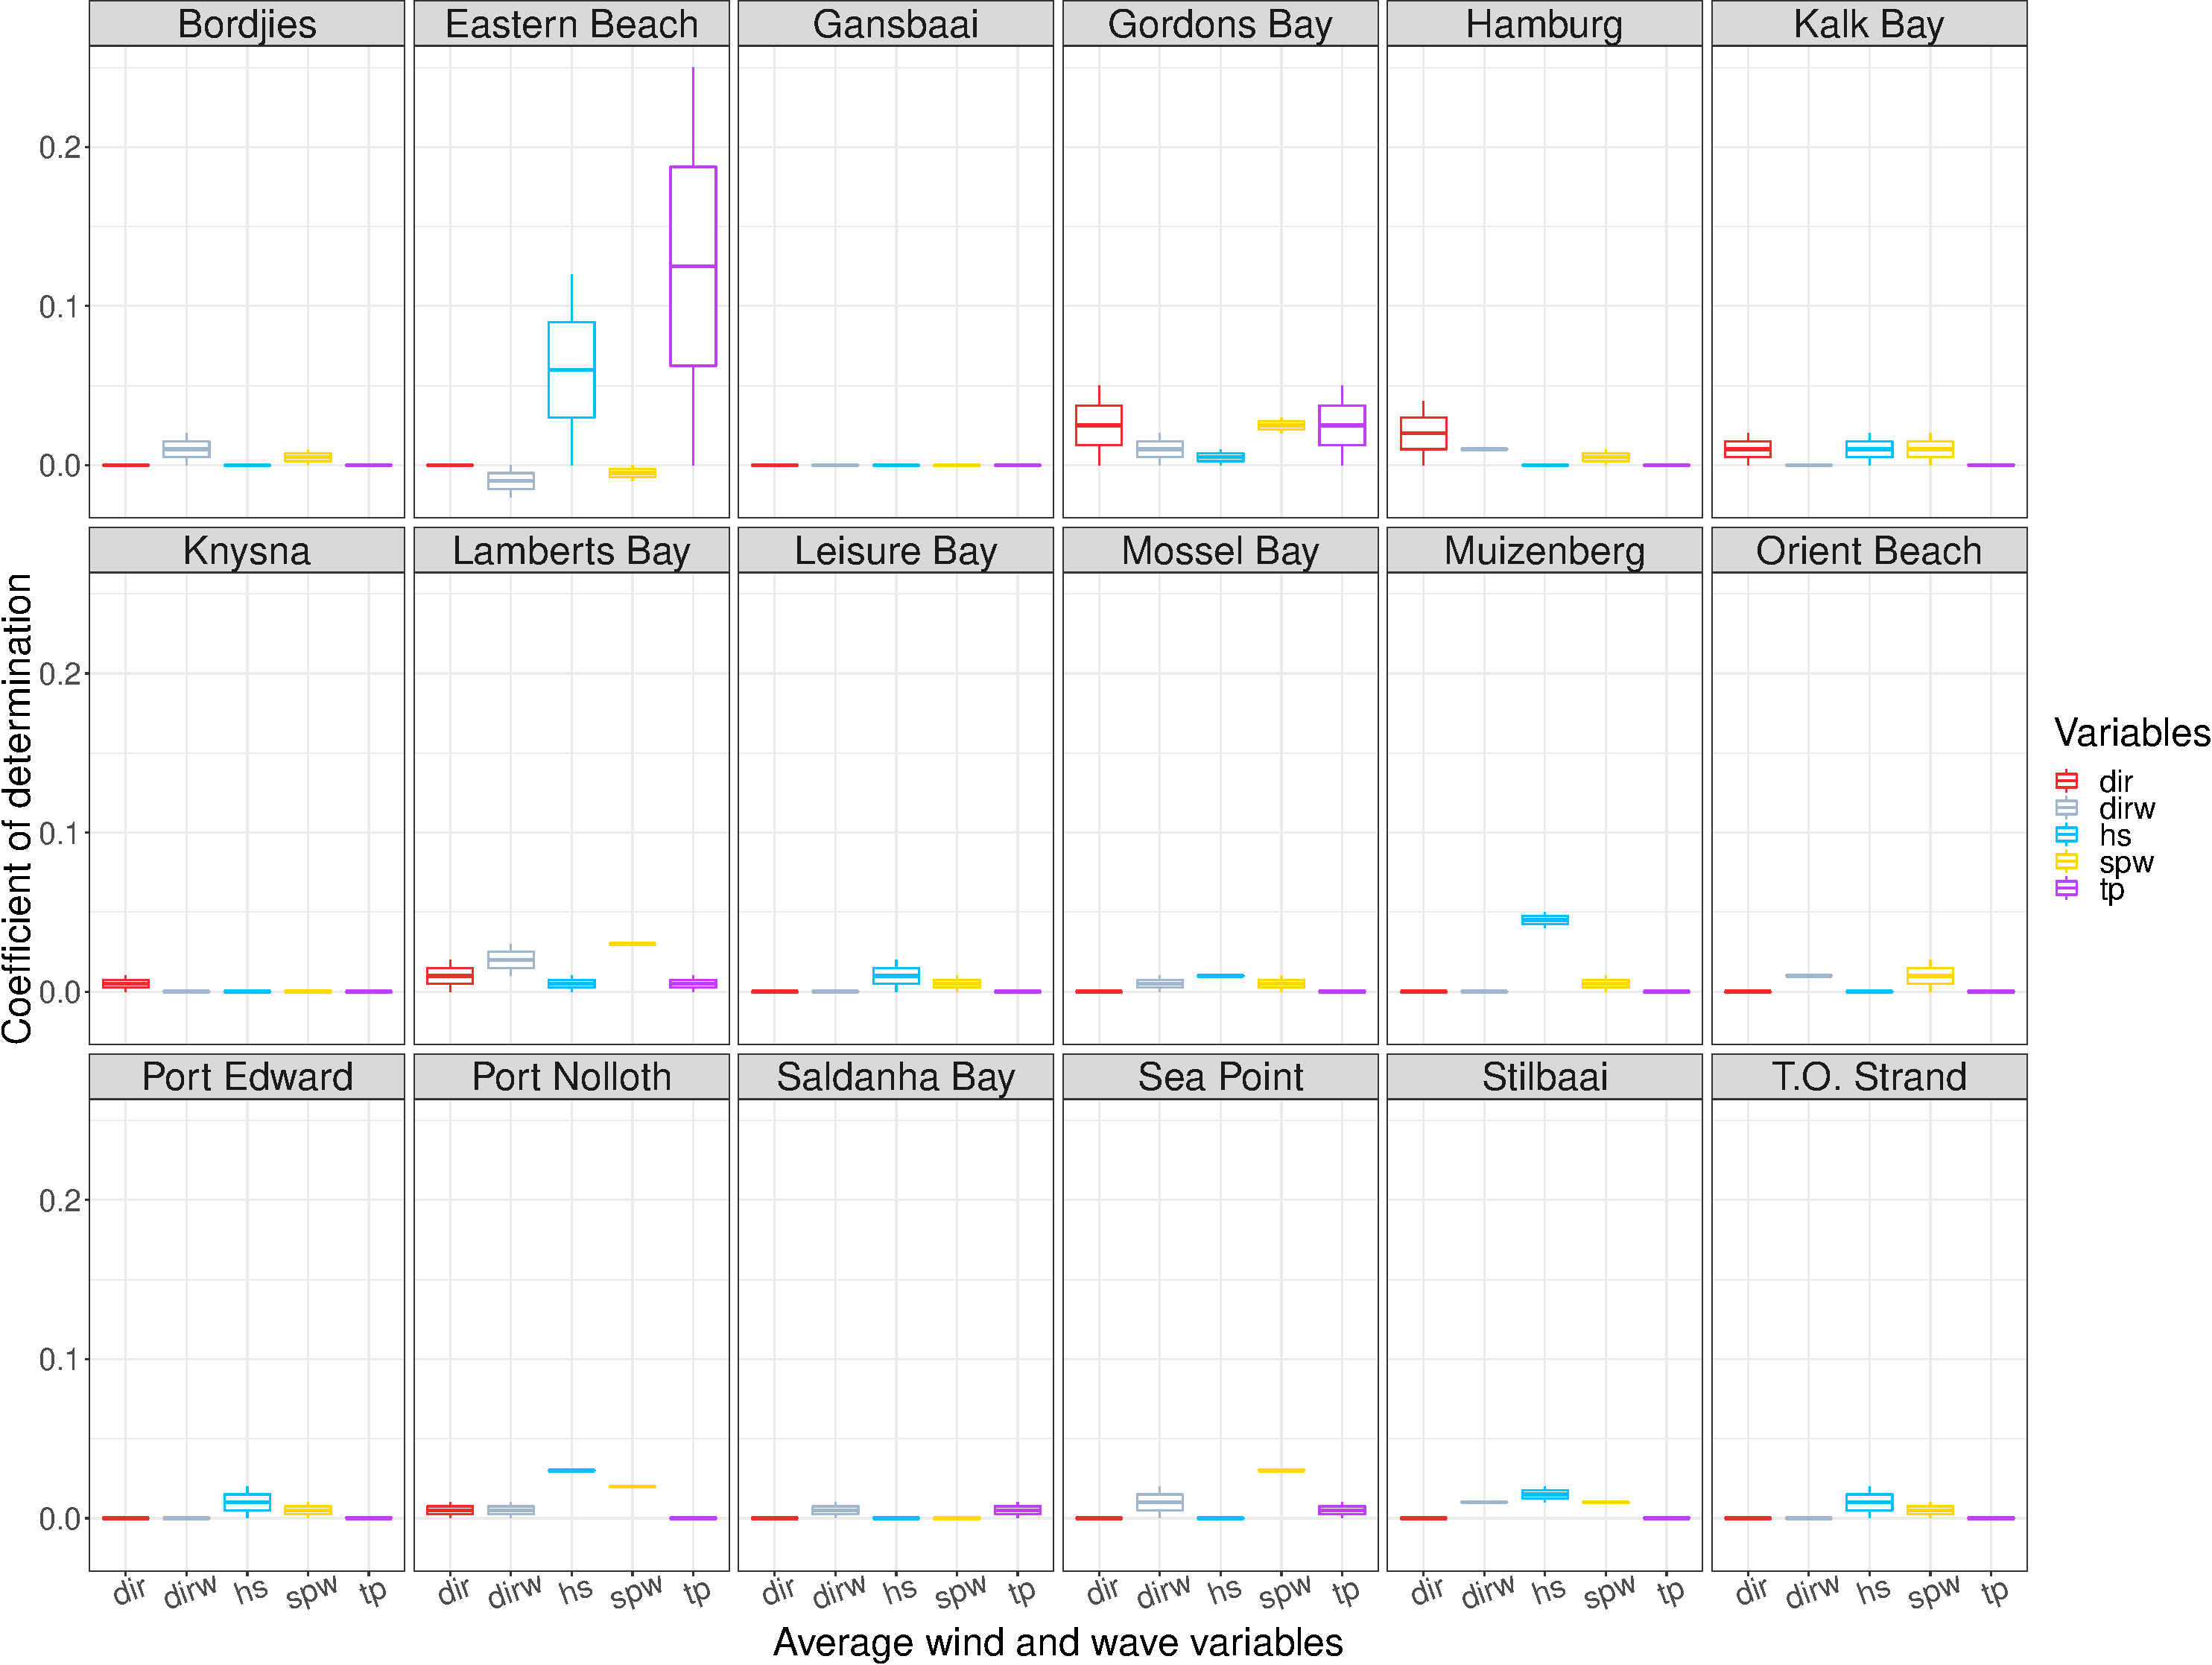
\includegraphics{appendices_files/figure-latex/Boxplot representing R2 values-1.pdf}

I now create a wind and wave rose diagram. Wind and wave diagrams help
visualise the patterns present at a particular site. Moving outward on
the radial scale, the frequency associated with wind and waves coming
from a partiular direction increases. Here I create a function to create
snooty wind and wave plots. As before the functions are ran in the setup
chunk of code at the begining of this document.

\begin{Shaded}
\begin{Highlighting}[]
\CommentTok{# source("functions/wind.rose.R")}

\CommentTok{# Now for creating the wind rose diagram}

\NormalTok{wave_daily_renamed <-}\StringTok{ }\NormalTok{wave_daily }\OperatorTok\StringTok{ }
\StringTok{  }\NormalTok{dplyr}\OperatorTok{::}\KeywordTok{rename}\NormalTok{(}\DataTypeTok{spd =}\NormalTok{ spw_mean) }\OperatorTok
\StringTok{  }\NormalTok{dplyr}\OperatorTok{::}\KeywordTok{rename}\NormalTok{(}\DataTypeTok{dir =}\NormalTok{ dirw_mean) }

\NormalTok{p.wr2 <-}\StringTok{ }\KeywordTok{plot.windrose}\NormalTok{(}\DataTypeTok{data =}\NormalTok{ wave_daily_renamed,}
              \DataTypeTok{spd =} \StringTok{"spd"}\NormalTok{,}
              \DataTypeTok{dir =} \StringTok{"dir"}\NormalTok{)}
\end{Highlighting}
\end{Shaded}

\begin{verbatim}
## Hadley broke my code
\end{verbatim}

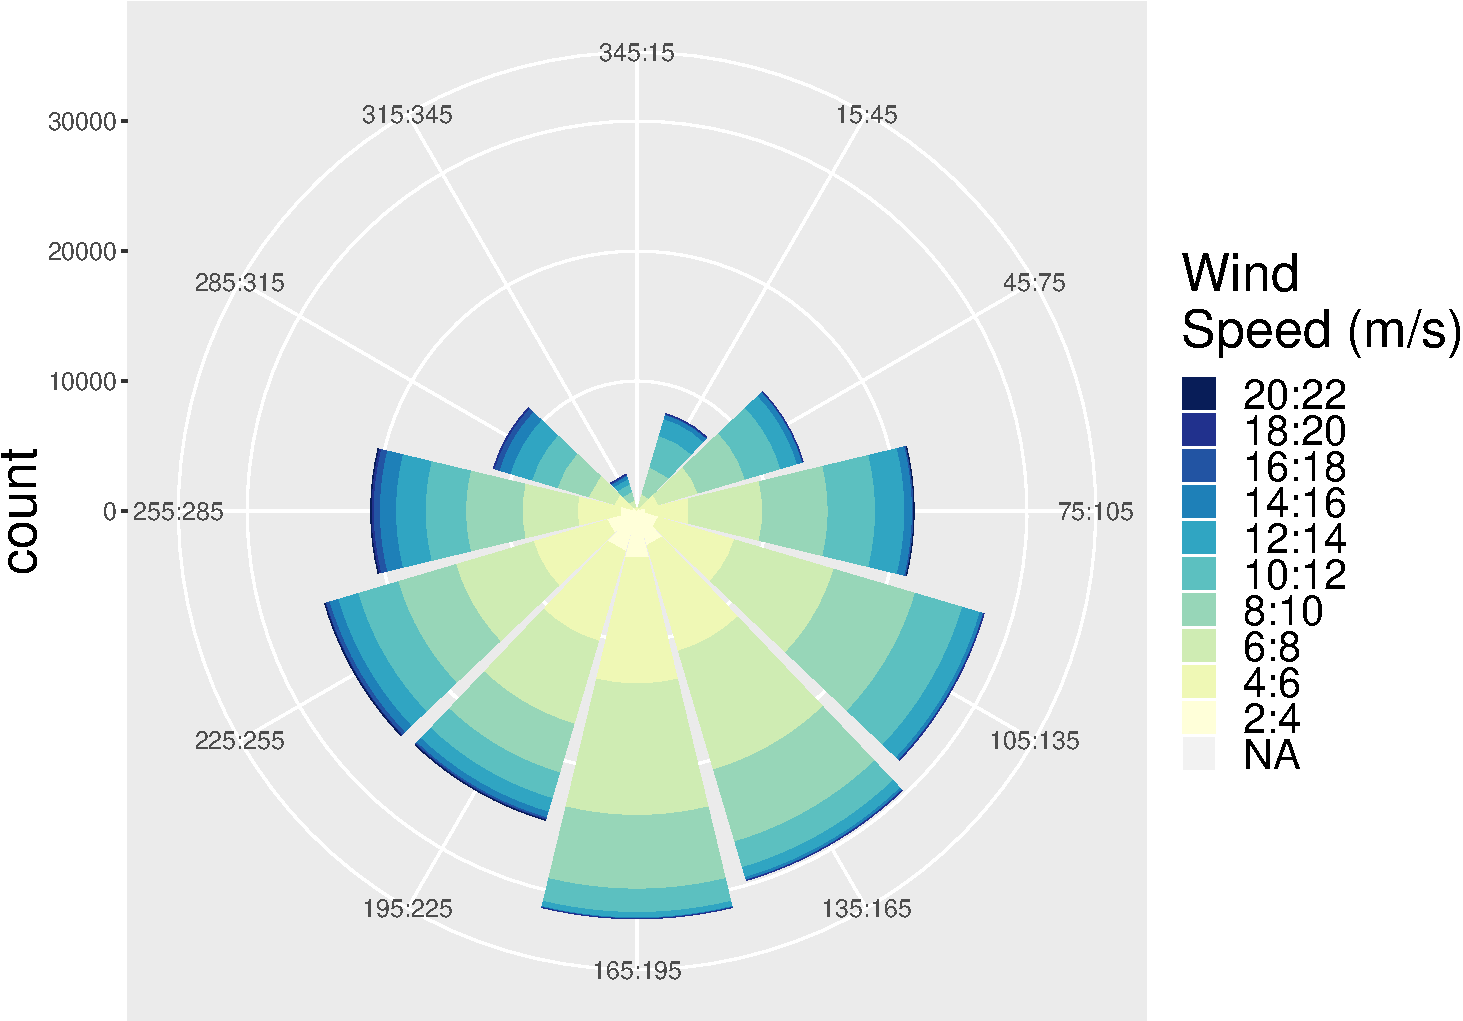
\includegraphics{appendices_files/figure-latex/Windrose diagram -1.pdf}

\begin{Shaded}
\begin{Highlighting}[]
\NormalTok{p.wr3 <-}\StringTok{ }\NormalTok{p.wr2 }\OperatorTok{+}\StringTok{ }\KeywordTok{facet_wrap}\NormalTok{(.}\OperatorTok{~}\StringTok{ }\NormalTok{site, }\DataTypeTok{ncol =} \DecValTok{4}\NormalTok{, }\DataTypeTok{nrow =} \DecValTok{5}\NormalTok{) }\OperatorTok{+}
\StringTok{  }\KeywordTok{theme}\NormalTok{(}\DataTypeTok{strip.text.x =} \KeywordTok{element_text}\NormalTok{(}\DataTypeTok{size =} \DecValTok{25}\NormalTok{))}
\NormalTok{p.wr3}
\end{Highlighting}
\end{Shaded}

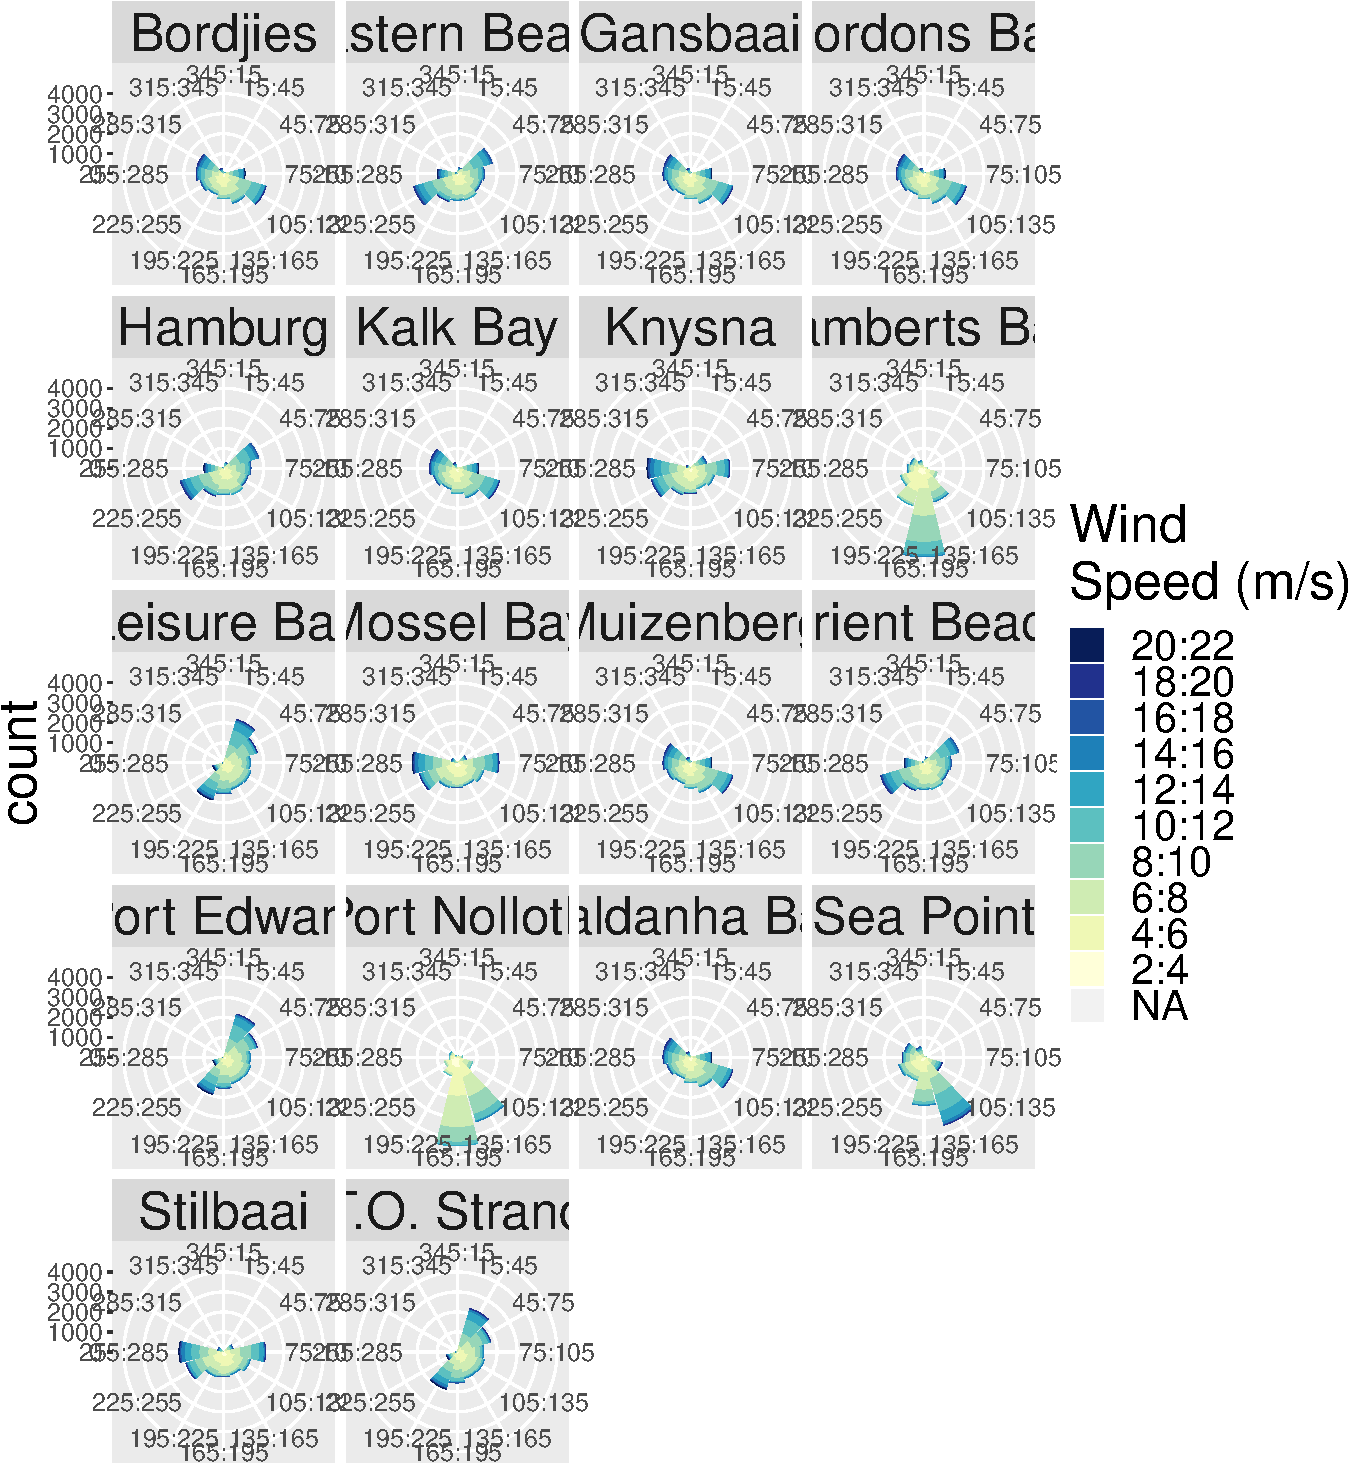
\includegraphics{appendices_files/figure-latex/Windrose diagram -2.pdf}

\begin{Shaded}
\begin{Highlighting}[]
\CommentTok{# ggsave(plot = p.wr3, filename = "figures/p.wr3.png")}
\end{Highlighting}
\end{Shaded}

Now for visualising the wave rose diagram

\begin{Shaded}
\begin{Highlighting}[]
\CommentTok{# source("functions/waverose.diagram.R")}

\CommentTok{# Now for creating the wave rose diagram}

\NormalTok{wave_daily_renamed <-}\StringTok{ }\NormalTok{wave_daily }\OperatorTok\StringTok{ }
\StringTok{  }\NormalTok{dplyr}\OperatorTok{::}\KeywordTok{rename}\NormalTok{(}\DataTypeTok{spd =}\NormalTok{ hs_mean) }\OperatorTok
\StringTok{  }\NormalTok{dplyr}\OperatorTok{::}\KeywordTok{rename}\NormalTok{(}\DataTypeTok{dir =}\NormalTok{ dir_mean) }

\NormalTok{p.wr2 <-}\StringTok{ }\KeywordTok{plot.waverose}\NormalTok{(}\DataTypeTok{data =}\NormalTok{ wave_daily_renamed,}
              \DataTypeTok{spd =} \StringTok{"spd"}\NormalTok{,}
              \DataTypeTok{dir =} \StringTok{"dir"}\NormalTok{) }
\end{Highlighting}
\end{Shaded}

\begin{verbatim}
## Warning in brewer.pal(min(max(0, n.colors.in.range), min(2, n.colors.in.range)), : minimal value for n is 3, returning requested palette with 3 different levels
\end{verbatim}

\begin{verbatim}
## Hadley broke my code
\end{verbatim}

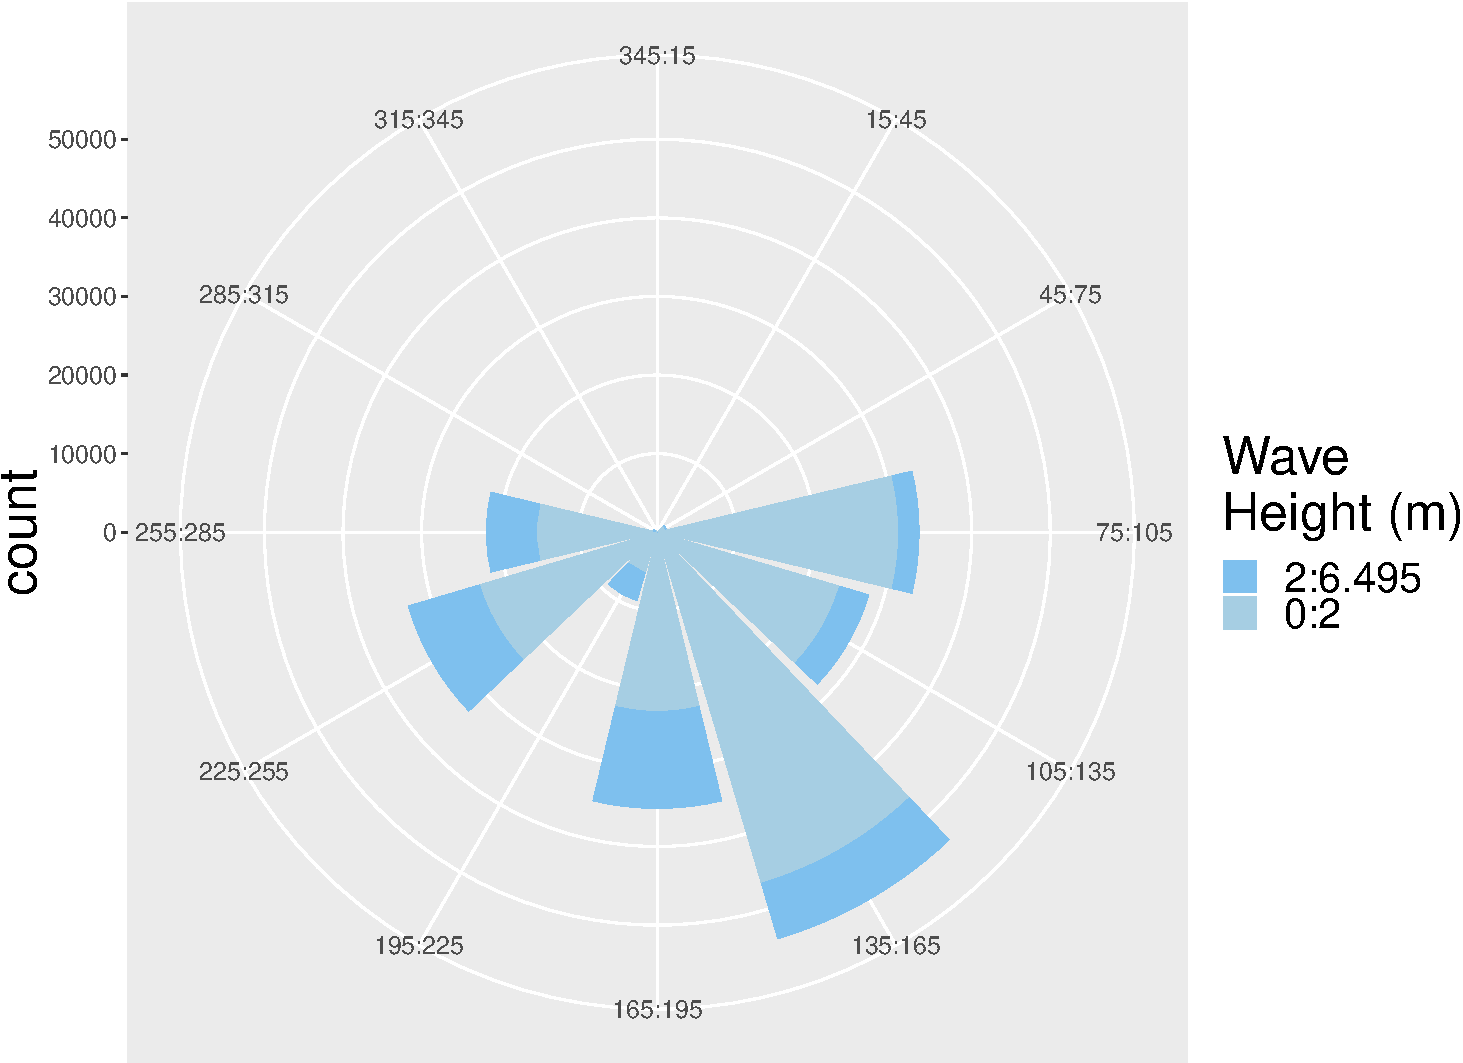
\includegraphics{appendices_files/figure-latex/Waverose diagram -1.pdf}

\begin{Shaded}
\begin{Highlighting}[]
\NormalTok{p.wr2}
\end{Highlighting}
\end{Shaded}

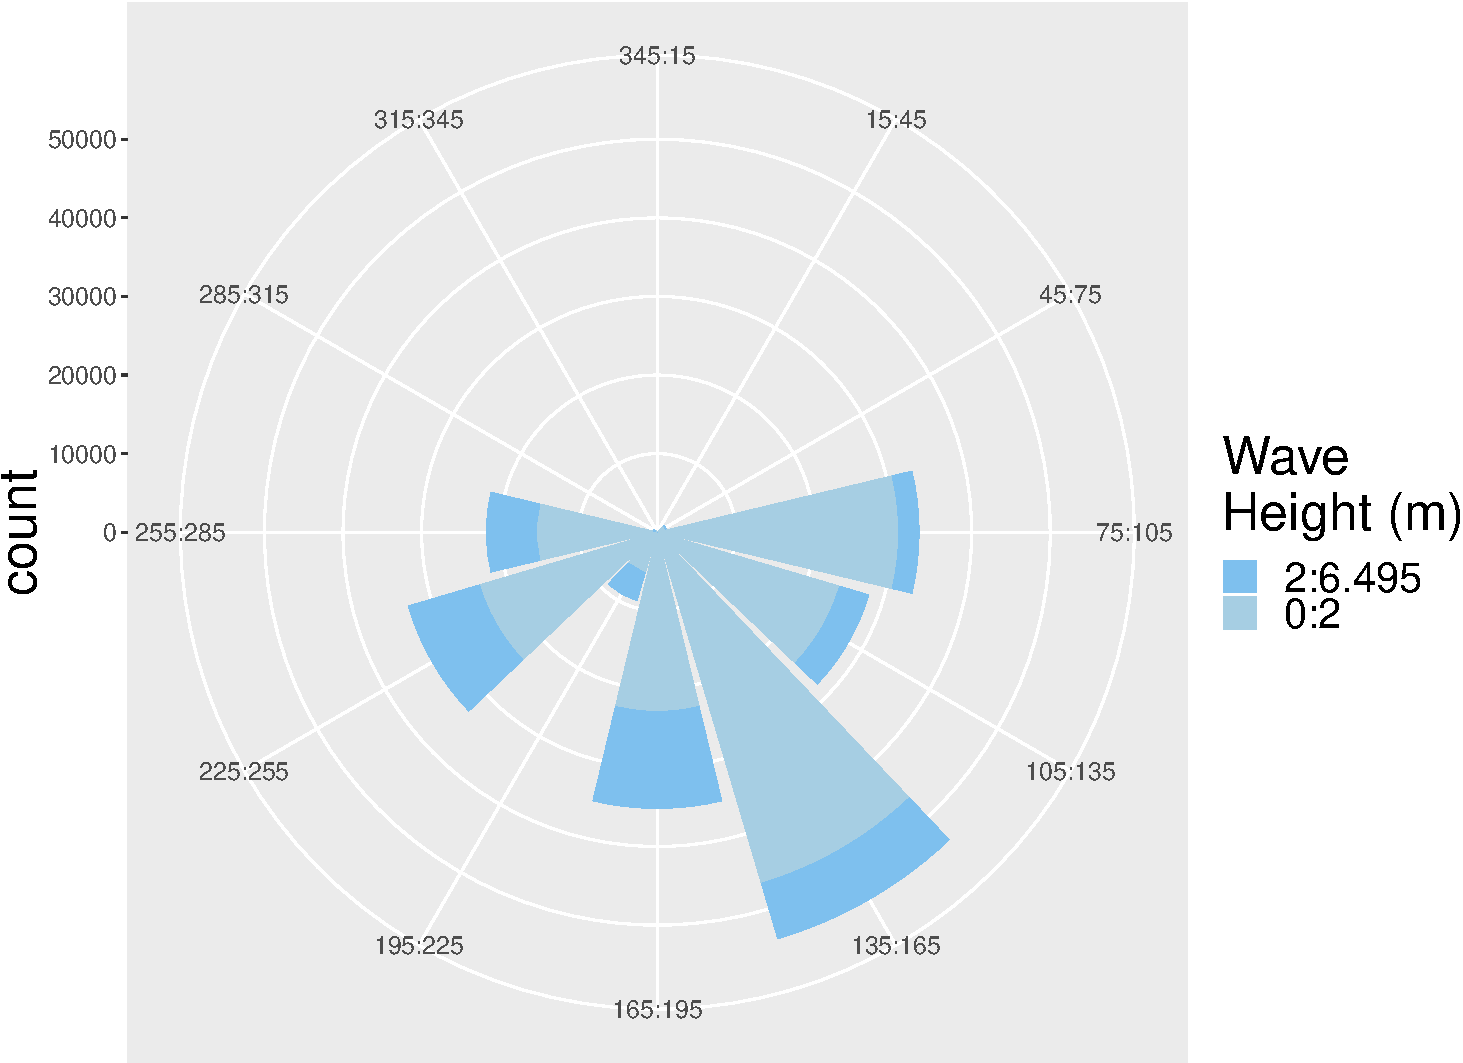
\includegraphics{appendices_files/figure-latex/Waverose diagram -2.pdf}

\begin{Shaded}
\begin{Highlighting}[]
\NormalTok{p.wave <-}\StringTok{ }\NormalTok{p.wr2 }\OperatorTok{+}\StringTok{ }\KeywordTok{facet_wrap}\NormalTok{(}\OperatorTok{~}\NormalTok{site,}
                            \DataTypeTok{ncol =} \DecValTok{6}\NormalTok{, }\DataTypeTok{nrow =} \DecValTok{3}\NormalTok{)}
\NormalTok{p.wave}
\end{Highlighting}
\end{Shaded}

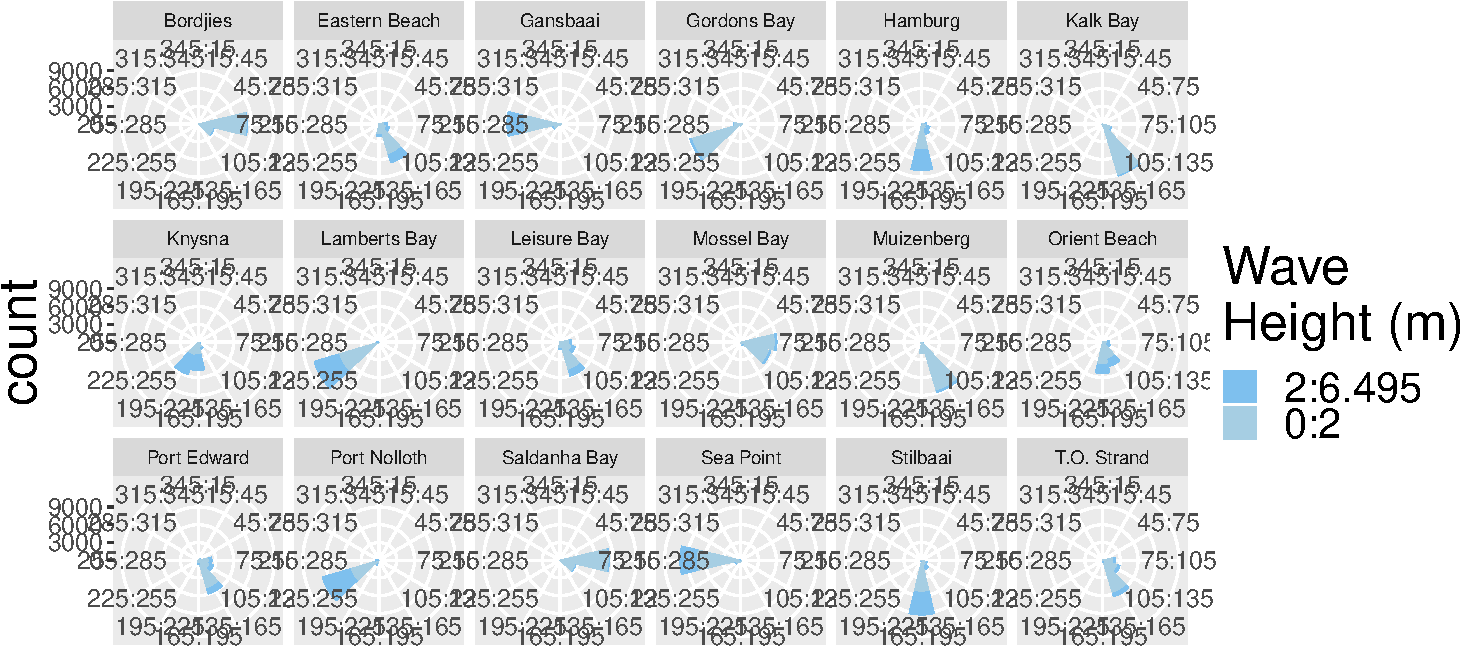
\includegraphics{appendices_files/figure-latex/Waverose diagram -3.pdf}

\begin{Shaded}
\begin{Highlighting}[]
\CommentTok{# ggsave(plot = p.wave, filename = "figures/p.wave.pdf")}
\end{Highlighting}
\end{Shaded}

\hypertarget{refs}{}
\hypertarget{ref-Mead2013}{}
Mead, A, CL Griffiths, GM Branch, CD McQuaid, LK Blamey, JJ Bolton, RJ
Anderson, et al. 2013. ``Human-Mediated Drivers of Change---impacts on
Coastal Ecosystems and Marine Biota of South Africa.'' \emph{African
Journal of Marine Science} 35 (3). Taylor \& Francis: 403--25.

\hypertarget{ref-Smit2017}{}
Smit, Albertus J, John J Bolton, and Robert J Anderson. 2017. ``Seaweeds
in Two Oceans: Beta-Diversity.'' \emph{Frontiers in Marine Science} 4.
Frontiers: 404.

\hypertarget{ref-Smit2013}{}
Smit, Albertus J, Michael Roberts, Robert J Anderson, Francois Dufois,
Sheldon FJ Dudley, Thomas G Bornman, Jennifer Olbers, and John J Bolton.
2013. ``A Coastal Seawater Temperature Dataset for Biogeographical
Studies: Large Biases Between in Situ and Remotely-Sensed Data Sets
Around the Coast of South Africa.'' \emph{PLoS One} 8 (12). Public
Library of Science: e81944.

\end{document}
